% =====================================================================
%  RAPORT NAUKOWO-BADAWCZY  --  Politechnika Poznanska
%  Wydzial Informatyki i Telekomunikacji
% ---------------------------------------------------------------------
%  Dokument: LEM - Location Encoding Model
%  Autor:    mgr Piotr Augustyniak
%
%  Raport naukowo-badawczy - material roboczy stanowiacy podstawe do
%  przygotowania fragmentow rozprawy i/lub artykulow naukowych.
%
%  Bazowy szablon:  PUT Dissertation Template (ppfcmthesis.cls,
%                   Weiss/Wesolek) - dostosowany do raportu.
%  Kompilator:  pdfLaTeX   |   Bibliografia: BibTeX
%
%  UWAGA: klasa ppfcmthesis.cls NIE jest modyfikowana - cala
%  personalizacja odbywa sie w tej preambule.
% =====================================================================

% --- Klasa ------------------------------------------------------------
\documentclass[polish,a4paper,oneside]{ppfcmthesis}

% --- Kodowanie i czcionki (pdfLaTeX) ---------------------------------
\usepackage[T1]{fontenc}
\usepackage[utf8]{inputenc}
\usepackage{lmodern}

% --- Pakiety uzywane w biezacej tresci ------------------------------
\usepackage{enumitem}    % listy (itemize / description)
\usepackage{float}       % pozycjonowanie rysunkow [H]
\usepackage{microtype}   % drobne poprawki typografii
\usepackage{tabularx}
\usepackage{longtable}
\usepackage{fvextra}
\usepackage{tikz}
\usetikzlibrary{positioning,arrows.meta,fit}
\RecustomVerbatimEnvironment{verbatim}{Verbatim}{breaklines=true,breakanywhere=true,fontsize=\small}
\setlength{\emergencystretch}{2em}
% (graphicx do \includegraphics jest juz ladowany przez klase)

% =====================================================================
% OPCJONALNY ZESTAW - odkomentuj wg potrzeb, gdy tresc tego wymaga.
% Celowo wylaczony, aby preambula zawierala tylko to, co aktualnie uzywane.
% =====================================================================
% --- Matematyka -----------------------------------------------------
% \usepackage{amsmath,amssymb}
%
% --- Tabele (rozszerzone) -------------------------------------------
% \usepackage{array}
% \usepackage{tabularx}
% \usepackage{multirow}
% \usepackage{longtable}
% \usepackage{colortbl}
% \newcolumntype{Y}{>{\raggedright\arraybackslash}X}
%
% --- Diagramy i wykresy ---------------------------------------------
% \usepackage{tikz}
% \usetikzlibrary{positioning,arrows.meta,fit,backgrounds,calc,shapes.geometric}
% \usepackage{pgfplots}
% \pgfplotsset{compat=1.18}
%
% --- Rysunki skladane (subfigure) -----------------------------------
% \usepackage{subcaption}
%
% --- Listingi kodu --------------------------------------------------
% \usepackage{listings}
% \usepackage{xcolor}
% \definecolor{kw}{RGB}{0,0,180}
% \definecolor{cm}{RGB}{60,140,60}
% \definecolor{str}{RGB}{160,40,40}
% \lstset{
%   basicstyle=\ttfamily\small,
%   keywordstyle=\color{kw}\bfseries, commentstyle=\color{cm}\itshape,
%   stringstyle=\color{str}, numbers=left, numberstyle=\tiny\color{gray},
%   frame=single, breaklines=true, tabsize=2, showstringspaces=false,
%   captionpos=b, inputencoding=utf8, extendedchars=true,
%   literate={ą}{{\k a}}1 {ć}{{\'c}}1 {ę}{{\k e}}1 {ł}{{\l}}1 {ń}{{\'n}}1
%            {ó}{{\'o}}1 {ś}{{\'s}}1 {ź}{{\'z}}1 {ż}{{\.z}}1
%            {Ą}{{\k A}}1 {Ć}{{\'C}}1 {Ę}{{\k E}}1 {Ł}{{\L}}1 {Ń}{{\'N}}1
%            {Ó}{{\'O}}1 {Ś}{{\'S}}1 {Ź}{{\'Z}}1 {Ż}{{\.Z}}1}
%
% --- Symbole i znaczniki zmian (z dokumentu zrodlowego) --------------
% \usepackage{pifont}
% \newcommand{\cmark}{\ding{51}}
% \newcommand{\xmark}{\ding{55}}
% \newcommand{\UWAGA}[1]{\textcolor{orange}{\small[\textbf{UWAGA:} #1]}}
% \newcommand{\dopis}[1]{\textcolor{red}{#1}}    % tresc nowa
% \newcommand{\zmiana}[1]{\textcolor{blue}{#1}}  % przeredagowania
% =====================================================================

% =====================================================================
% NUMERACJA WG KONWENCJI POLSKIEJ - kropka po ostatnim numerze
% =====================================================================
% Efekt: "1.1. Wprowadzenie", "Rysunek 1.1. Tytul", "Tabela 1.1. Tytul".
% Numer rozdzialu (pierwszy poziom) - bez kropki.
%
% UWAGA TYPOGRAFICZNA: w tej konwencji \ref zwraca numer Z KROPKA
% (np. "2.1."). Nie konczyc zdan na \ref (powstanie podwojna kropka).
% ---------------------------------------------------------------------
\renewcommand{\thesection}{\thechapter.\arabic{section}.}
\renewcommand{\thesubsection}{\thechapter.\arabic{section}.\arabic{subsection}.}
\renewcommand{\thesubsubsection}{\thechapter.\arabic{section}.\arabic{subsection}.\arabic{subsubsection}.}

% Patch running header - po zmianie \thesection unikamy podwojnej kropki
% w zywej paginie (nadpisany tylko \sectionmark).
\makeatletter
\renewcommand{\@ppfcmthesismarks}{%
  \let\@mkboth\markboth
  \def\chaptermark##1{\markboth{##1}{##1}}%
  \def\sectionmark##1{\markright{%
    \ifnum \c@secnumdepth>\z@
      \thesection\ %
    \fi
    ##1}}%
  \def\tocmark{\markboth{\contentsname}{}}%
  \def\lofmark{\markboth{\listfigurename}{}}%
  \def\lotmark{\markboth{\listtablename}{}}%
  \def\bibmark{\markboth{\bibname}{}}%
  \def\indexmark{\markboth{\indexname}{}}%
}
\makepsmarks{ppfcmthesis}{\@ppfcmthesismarks}
\makeatother

\renewcommand{\thefigure}{\thechapter.\arabic{figure}.}
\renewcommand{\thetable}{\thechapter.\arabic{table}.}

% Podpisy rysunkow/tabel - pakiet caption + przekierowanie makr klasy
% (\fcmfcaption pod rysunkiem, \fcmtcaption nad tabela) na zwykly \caption.
\usepackage{caption}
\captionsetup{labelformat=simple,labelsep=space,
              font={small},labelfont={small,bf}}
\makeatletter
\renewcommand{\fcmfcaption}[2][\@empty]{%
  \ifx\@empty#1\@empty \caption{#2}\else \caption[#1]{#2}\fi}
\renewcommand{\fcmtcaption}[2][\@empty]{%
  \ifx\@empty#1\@empty \caption{#2}\else \caption[#1]{#2}\fi}
\makeatother

% =====================================================================
% METADANE RAPORTU  --  EDYTUJ PONIZEJ
% =====================================================================
% Rodzaj dokumentu (naglowek nad tytulem):
\newcommand{\raporttyp}{Raport naukowo-badawczy}

% -----------------------------------------------------------------
% NUMER RAPORTU - schemat:  RP / <numer kolejny> / <rok> <JEZYK>
%   RP      - typ dokumentu (RaPort)
%   numer   - kolejny numer w danym roku (np. 01, 02, ...)
%   rok     - rok wydania
%   jezyk   - PL lub EN
% Przyklad: RP/01/2026 PL
% -----------------------------------------------------------------
\newcommand{\nrraportu}{RP/01/2026 PL}

% Podtytul / nazwa tematu badawczego (opcjonalny - zostaw pusty, jesli brak):
\newcommand{\podtytul}{}

% Tytul:
\newcommand{\tytulraportu}{LEM~--- Location Encoding Model}

% Autor (z tytulem naukowym/zawodowym):
\newcommand{\autor}{mgr Piotr Augustyniak}

% Grupa badawcza / afiliacja zespolu:
\newcommand{\grupabadawcza}{Grupa badawcza pod kierunkiem dr.~hab.~in\.z. Piotra Zwierzykowskiego, prof.~PP}

% Opiekun naukowy / kierownik projektu (opcjonalny - zostaw pusty, jesli brak):
\newcommand{\opiekun}{}

% Rok:
\newcommand{\rok}{2026}
\newcommand{\wersja}{1.0}
\newcommand{\statusraportu}{Preprint --- specyfikacja techniczna}
\newcommand{\datawydania}{13 wrze\'snia 2026}

\hypersetup{
  pdftitle={LEM - Location Encoding Model},
  pdfauthor={Piotr Augustyniak},
  pdfsubject={Raport naukowo-badawczy, nr RP/01/2026 PL},
  pdfkeywords={LEM, Location Encoding Model, lokalizacja, model semantyczny}
}

\begin{document}
\hypersetup{pageanchor=false}

% =====================================================================
% STRONA TYTULOWA
% =====================================================================
\frontmatter\pagestyle{empty}
\begin{titlingpage}
% Numer raportu - prawy gorny rog
\hfill{\small Nr\ \nrraportu}\par
\begin{center}
  
\includegraphics[width=0.9\textwidth]{figures/sygnet-pp.pdf}\\[1.2em]
  {\large Politechnika Pozna\'nska}\\[0.2em]
  Wydzia\l{} Informatyki i~Telekomunikacji\\
  Instytut Sieci Teleinformatycznych

  \vspace{2.0cm}

  {\Large\scshape \raporttyp}%
  \ifx\podtytul\empty\else\\[0.4em]{\large \podtytul}\fi

  \vspace{1.4cm}

  \rule{\textwidth}{0.4pt}\\[0.8em]
  {\LARGE\bfseries \tytulraportu}\\[0.8em]
  \rule{\textwidth}{0.4pt}

  \vspace{2.0cm}

  \begin{minipage}{0.85\textwidth}
    \large
    \begin{tabular}{@{}r@{\hspace{1.5em}}l@{}}
      \textbf{Autor:}          & \autor \\[0.6em]
      % Aby dodac opiekuna naukowego, odkomentuj ponizszy wiersz:
      % \textbf{Opiekun naukowy:} & \opiekun \\[0.6em]
      \textbf{Nr raportu:} & \nrraportu \\
      \textbf{Wersja:} & \wersja \\
      \textbf{Status:} & \statusraportu \\
      \textbf{Data:} & \datawydania \\
    \end{tabular}
  \end{minipage}

  \vspace{1.0cm}

  {\large \grupabadawcza}

  \vfill

  \begin{minipage}{0.9\textwidth}
    \centering\footnotesize
    \textcopyright{} 2026 Piotr Augustyniak. Treść raportu oraz autorskie
    tabele i diagramy: CC BY 4.0. Artefakty techniczne: Apache License 2.0.
    Logotypy PP, klasa szablonu i materiały osób trzecich są wyłączone.
  \end{minipage}

  \vspace{0.8em}

  Pozna\'n, \rok
\end{center}
\end{titlingpage}
\cleardoublepage
\hypersetup{pageanchor=true}
\pagenumbering{Roman}

% % =====================================================================
% % STRESZCZENIE  (tresc 1:1 z abstraktu dokumentu zrodlowego)
% % =====================================================================
% \thispagestyle{empty}
% \section*{Streszczenie}
% \addcontentsline{toc}{chapter}{Streszczenie}
% Niniejszy dokument definiuje Model Kodowania Lokalizacji (\textit{Location Encoding Model} – LEM) — hierarchiczny, rozszerzalny model semantyczny do reprezentacji fizycznej lokalizacji urządzeń infrastruktury sieciowej w przestrzeniach wewnętrznych i pół-otwartych. LEM wprowadza ujednolicony sposób opisu lokalizacji, niezależny od producenta sprzętu, stosowanego protokołu oraz przyjętej konwencji nazewniczej. Model umożliwia reprezentację lokalizacji na różnych poziomach szczegółowości i w wielu formatach — od czytelnego dla człowieka ciągu znaków, przez strukturyzowane dane, po zwarte kodowanie binarne. Celem LEM jest ułatwienie zarządzania infrastrukturą, automatyzacji procesów operacyjnych, integracji systemów oraz zapewnienie deterministycznego i jednoznacznego opisu lokalizacji urządzeń w środowiskach \textit{enterprise}, kampusowych, przemysłowych i OT. Dokument określa model danych, zasady kodowania i interpretacji, mechanizmy rozszerzania oraz przykładowe mapowania do istniejących protokołów i technologii sieciowych.
% \vfill\cleardoublepage

% =====================================================================
% STRESZCZENIE  (tresc 1:1 z abstraktu dokumentu zrodlowego)
% =====================================================================
\thispagestyle{empty}
\section*{Streszczenie}
\addcontentsline{toc}{chapter}{Streszczenie}
Niniejszy dokument definiuje Model Kodowania Lokalizacji (\textit{Location Encoding Model}, LEM) --- niewielki, niezależny od reprezentacji model informacji o lokalizacji. LEM określa pięć komponentów opisu lokalizacji encji, ich dziedziny wartości, reguły spójności oraz deterministyczną postać kanoniczną. Reprezentacje tekstowe, JSON, binarne TLV i YANG odwzorowują ten sam rdzeń semantyczny; mapowania do Civic Address i GeoJSON ilustrują integrację z istniejącymi modelami. Stratny zapis DNS-safe jest jawnie klasyfikowany jako alias prezentacyjny, a nie równoważna reprezentacja LEM. Profile zastosowań mogą nakładać dodatkowe wymagania bez zmiany podstawowej semantyki modelu. Dokument obejmuje także zasady implementacji, bezpieczeństwa, prywatności, wersjonowania oraz zestaw walidowalnych artefaktów referencyjnych.
\vfill\cleardoublepage

\thispagestyle{empty}
\section*{Abstract}
\addcontentsline{toc}{chapter}{Abstract}
This document specifies the Location Encoding Model (LEM), a compact, representation-independent information model for describing the physical location of an entity. LEM defines five components, their value domains, consistency constraints, and a deterministic canonical form. Text, JSON, binary TLV, and YANG representations map to the same semantic core; mappings to Civic Address and GeoJSON illustrate integration with established models. A lossy DNS-safe form is explicitly classified as a presentation alias rather than a semantically equivalent LEM representation. Application profiles may impose additional requirements without changing the core semantics. The specification also covers implementation, security, privacy, versioning, and machine-verifiable reference artefacts.
\vfill\cleardoublepage



% --- Spis tresci (automatyczny) -------------------------------------
\pagestyle{ppfcmthesis}
\tableofcontents*
\cleardoublepage

% % =====================================================================
% % TRESC
% % =====================================================================
% \mainmatter
% \renewcommand{\thefigure}{\thechapter.\arabic{figure}.}
% \renewcommand{\thetable}{\thechapter.\arabic{table}.}

% % =====================================================================
% Rozdzial 1: Wprowadzenie
% =====================================================================

\chapter{Wprowadzenie}
\label{chap:wprowadzenie}

\section{Cel modelu LEM}
\label{sec:cel-lem}
Informacja o lokalizacji jest wykorzystywana przez wiele systemów technicznych działających w różnych domenach zastosowań. Systemy zarządzania infrastrukturą, automatyzacji, bezpieczeństwa, dokumentacji technicznej oraz usług lokalizacyjnych wymagają jednoznacznego opisu położenia obiektów fizycznych. W praktyce informacje te są często reprezentowane przy użyciu lokalnych konwencji zależnych od systemu, producenta lub technologii. Stosowane podejścia obejmują między innymi:

\begin{itemize}
    \item nieustrukturyzowane opisy tekstowe w systemach CMDB, bazach danych lub dokumentacji technicznej,
    \item lokalne schematy nazewnictwa urządzeń i przestrzeni,
    \item oznaczenia wynikające z dokumentacji architektonicznej lub organizacyjnej,
    \item informacje utrzymywane jako wiedza operacyjna określonych osób lub zespołów.
\end{itemize}

Takie sposoby opisu często nie zapewniają jednoznacznej, deterministycznej i maszynowo interpretowalnej informacji. Konsekwencją braku wspólnego modelu semantycznego są m.in. ograniczona interoperacyjność, utrudniona automatyzacja oraz problemy z utrzymaniem spójności.

Model Kodowania Lokalizacji (\textit{Location Encoding Model}, LEM) definiuje wspólny model semantyczny, którego celem jest zapewnienie jednoznacznego znaczenia komponentów niezależnie od sposobu ich reprezentacji czy implementacji. LEM definiuje znaczenie informacji, podczas gdy sposób jej wyrażenia w konkretnym formacie pozostaje warstwą niezależną.

\section{Zakres dokumentu}
\label{sec:zakres}
Niniejszy dokument definiuje \textit{Location Encoding Model} (LEM) jako model informacji przeznaczony do opisu lokalizacji. Specyfikacja określa:

\begin{itemize}
    \item model semantyczny informacji o lokalizacji,
    \item komponenty modelu LEM oraz ich znaczenie,
    \item zasady interpretacji informacji, równoważności semantycznej oraz spójności modelu,
    \item zasady reprezentacji informacji LEM oraz tworzenia profili zastosowań.
\end{itemize}

Dokument nie definiuje formatów wymiany danych, protokołów komunikacyjnych, technologii pomiaru lokalizacji, algorytmów pozycjonowania ani wymagań specyficznych dla pojedynczego środowiska.

LEM nie definiuje mechanizmów identyfikacji obiektów, pozyskiwania informacji lokalizacyjnej ani metod określania położenia. Model opisuje wyłącznie semantykę informacji o lokalizacji już dostępnej.

\section{Wkład dokumentu}
\label{sec:wklad}
Wkład LEM obejmuje cztery elementy:
\begin{enumerate}
    \item niewielki rdzeń semantyczny oddzielający znaczenie lokalizacji od jej reprezentacji;
    \item deterministyczną postać kanoniczną i jawne reguły równoważności opisów częściowych;
    \item spójne odwzorowania na JSON, TLV i YANG oraz mapowania integracyjne do Civic Address i GeoJSON;
    \item mechanizm profili umożliwiający specjalizację domenową bez redefiniowania rdzenia modelu.
\end{enumerate}

\section{Niezależność semantyki od reprezentacji}
\label{sec:niezaleznosc}
Model LEM rozdziela znaczenie informacji od sposobu jej wyrażenia. Znaczenie jest określone przez model semantyczny i interpretację kanoniczną. Ta sama informacja może być wyrażona w różnych reprezentacjach (tekstowej, strukturalnej, binarnej), które są semantycznie równoważne, jeśli prowadzą do tej samej interpretacji zgodnie z zasadami LEM.

\section{Struktura dokumentu}
\label{sec:struktura-dok}
\begin{description}
    \item[Rozdział 2:] Definiuje model semantyczny LEM, komponenty oraz zasady interpretacji.
    \item[Rozdział 3:] Definiuje zasady reprezentacji modelu w różnych formatach danych.
    \item[Rozdział 4:] Definiuje profile zastosowań dla specjalizacji domenowych.
    \item[Rozdziały 5--7:] Omawiają implementację, bezpieczeństwo, prywatność i ewolucję modelu.
    \item[Rozdział 8:] Osadza LEM względem istniejących standardów i modeli.
\end{description}

\section{Terminologia i konwencje}
\label{sec:terminologia}
Na potrzeby dokumentu przyjęto następujące definicje:

\begin{description}
    \item[Model informacji (\textit{Information Model}):] Abstrakcyjny model definiujący strukturę, znaczenie oraz relacje elementów.
    \item[Informacja o lokalizacji:] (\textit{Location Information}) Informacja opisana przy użyciu komponentów LEM.
    \item[Komponent modelu (\textit{Model Component}):] Element LEM posiadający znaczenie semantyczne.
    \item[Przestrzeń referencyjna (\textit{Reference Space}):] Przestrzeń odniesienia dla interpretacji przestrzennej.
    \item[Położenie względne (\textit{Relative Position}):] Relacja przestrzenna względem przestrzeni referencyjnej.
    \item[Reprezentacja (\textit{Representation}):] Sposób wyrażenia informacji przy użyciu formatu danych.
    \item[Interpretacja kanoniczna (\textit{Canonical Interpretation}):] Jednoznaczne znaczenie wynikające z modelu LEM.
    \item[Profil LEM (\textit{LEM Profile}):] Specjalizacja modelu określająca wymagania dla danego zastosowania.
\end{description}

Słowa kluczowe zapisane wielkimi literami są używane zgodnie z BCP~14 \cite{RFC2119,RFC8174}: \textbf{MUSI} odpowiada \textit{MUST}, \textbf{NIE MOŻE} --- \textit{MUST NOT}, \textbf{POWINIEN} --- \textit{SHOULD}, a \textbf{MOŻE} --- \textit{MAY}. Przykłady mają charakter ilustracyjny, o ile nie oznaczono ich inaczej.

% % =====================================================================
% Rozdział 2: Model semantyczny LEM
% =====================================================================

\chapter{Model semantyczny LEM}
\label{chap:model}

\section{Komponenty modelu}
\label{sec:komponenty}
\textit{Location} jest logiczną kompozycją komponentów semantycznych opisujących fizyczną lokalizację obiektu. Poszczególne komponenty dostarczają informacji o różnych aspektach lokalizacji i mogą występować niezależnie od siebie, z uwzględnieniem ograniczeń określonych w niniejszej specyfikacji.

Model LEM definiuje zestaw komponentów semantycznych służących do opisu fizycznej lokalizacji obiektu. Każdy komponent reprezentuje określony aspekt informacji lokalizacyjnej i posiada niezależną semantykę. Komponenty mogą być stosowane pojedynczo lub łączone w celu uzyskania większego poziomu szczegółowości opisu lokalizacji.

\begin{figure}[htbp]
\centering
\begin{tikzpicture}[node distance=9mm and 8mm,
  box/.style={draw,rounded corners,align=center,minimum width=25mm,minimum height=8mm},
  arr/.style={-{Latex[length=2mm]},thick}]
  \node[box] (entity) {Encja};
  \node[box,right=of entity] (location) {Location};
  \node[box,below left=of location] (site) {Site};
  \node[box,below=of location] (building) {Building};
  \node[box,below right=of location] (level) {Level};
  \node[box,below=18mm of site] (ref) {Reference\\Space};
  \node[box,below=18mm of level] (rel) {Relative\\Position};
  \draw[arr] (entity) -- (location);
  \draw[arr] (location) -- (site);
  \draw[arr] (location) -- (building);
  \draw[arr] (location) -- (level);
  \draw[arr] (location) -- (ref);
  \draw[arr] (location) -- (rel);
  \draw[arr,dashed] (rel) -- node[below,sloped,font=\scriptsize]{względem} (ref);
\end{tikzpicture}
\caption{Rdzeń semantyczny modelu LEM}
\label{fig:lem-core}
\end{figure}

O ile niniejsza specyfikacja nie określa inaczej, brak komponentu oznacza brak określonej informacji, a nie wartość domyślną (zob. sekcja \ref{sec:opisy-czesciowe}).

Poniższe sekcje definiują znaczenie poszczególnych komponentów oraz podstawowe reguły ich wykorzystania. Zasady dotyczące zależności pomiędzy komponentami, wymagań minimalnych, walidacji semantycznej, przypadków niepełnej lokalizacji oraz konfliktu informacji są określone łącznie w sekcjach \ref{sec:kanoniczna-interpretacja} (Kanoniczna interpretacja) oraz \ref{sec:spojnosci-modelu} (Reguły spójności modelu).

\subsection{Site}
\label{sec:comp-site}
\textit{Site} --- najwyższy poziom hierarchii lokalizacji, definiowany przez implementację.

\subsection{Building}
\label{sec:comp-building}
\textit{Building} --- element hierarchii lokalizacji reprezentujący pojedynczy budynek lub inny wydzielony obiekt przestrzenny, definiowany przez implementację.

\subsection{Level}
\label{sec:comp-level}
\textit{Level} --- element hierarchii lokalizacji reprezentujący poziom przestrzeni, definiowany przez implementację.

\subsection{Reference Space}
\label{sec:comp-refspace}
\textit{Reference Space} --- jednoznacznie identyfikowalna przestrzeń stanowiąca punkt odniesienia do określenia położenia względnego obiektu.

\subsection{Relative Position}
\label{sec:comp-relpos}
\textit{Relative Position} --- opis położenia obiektu względem zdefiniowanej przestrzeni referencyjnej.

Znaczenie każdego komponentu oraz relacji pomiędzy nimi jest niezależne od reprezentacji, w której komponent został zapisany (zob. Rozdział 3).

\subsection{Formalne typy danych komponentów (normatywne)}
\label{sec:typy-danych}
Lokalizacja encji jest reprezentowana przez pięć niezależnych komponentów. Każdy komponent ma zdefiniowany typ i semantykę. Wartości tekstowe zawierają od 1 do 256 punktów kodowych Unicode. UTF-8 \cite{RFC3629} jest kodowaniem stosowanym przez wybrane reprezentacje, a nie miarą długości semantycznej.

\begin{description}
    \item[Site:]
    \begin{itemize}
        \item \textbf{Typ:} \texttt{string}
        \item \textbf{Semantyka:} nazwa lub identyfikator tekstowy miejsca/siedziby/kampusu, w obrębie którego znajduje się \textit{Building}.
        \item \textbf{Wymaganie:} komponent opcjonalny w modelu podstawowym; profil może wymagać jego obecności.
        \item \textbf{Uwaga projektowa (nie stanowi części modelu):} w przyszłych integracjach z systemami zewnętrznymi (CMDB, GIS) zaleca się rozróżnienie wartości prezentacyjnej (\texttt{name}) od stabilnego identyfikatora. Obecny model tego rozróżnienia nie wprowadza.
    \end{itemize}

    \item[Building:]
    \begin{itemize}
        \item \textbf{Typ:} \texttt{string}
        \item \textbf{Semantyka:} nazwa lub identyfikator tekstowy budynku (lub równoważnego obiektu budowlanego) znajdującego się w \textit{Site}.
        \item \textbf{Wymaganie:} komponent opcjonalny w modelu podstawowym.
        \item \textbf{Uwaga projektowa:} analogicznie do \textit{Site}.
    \end{itemize}

    \item[Level:]
    \begin{itemize}
        \item \textbf{Typ:} struktura \texttt{Level} z polami \texttt{kind} oraz \texttt{value}.
        \item \textbf{Semantyka:} 
        \begin{itemize}
            \item \texttt{kind = "numeric"} --- \texttt{value} jest wymagane i musi być liczbą całkowitą ze znakiem w zakresie od $-2^{31}$ do $2^{31}-1$. \texttt{0} oznacza poziom parteru / ground floor (konwencja modelu, niezależna od lokalnej numeracji źródłowej). Wartości dodatnie oznaczają kondygnacje nadziemne; wartości ujemne oznaczają kondygnacje podziemne.
            \item \texttt{kind = "non-building"} --- \texttt{value} musi być \texttt{null}. Oznacza, że encja nie znajduje się na żadnej kondygnacji budynku (dach, parking naziemny, przestrzeń zewnętrzna, strefa pomiędzy budynkami itp.). Przestrzeń taka jest w takim wypadku dalej opisywana przez \textit{Reference Space} (np. \texttt{"Roof"}), a nie przez \texttt{value}.
        \end{itemize}
        \item \textbf{Wymaganie:} komponent opcjonalny w modelu podstawowym.
        \item \textbf{Zakaz:} wartości ułamkowe oraz inne typy niż określone powyżej są niedozwolone. Przypadek antresoli pozostaje nieobsłużony przez model podstawowy.
    \end{itemize}

    \item[Reference Space:]
    \begin{itemize}
        \item \textbf{Typ:} \texttt{string}
        \item \textbf{Semantyka:} nazwana lub w inny sposób określona przestrzeń stanowiąca kontekst lokalizacyjny dla encji --- pomieszczenie, sala, pokój, korytarz, hala, parking, dach, strefa zewnętrzna lub inna przestrzennie znacząca jednostka. \textit{Reference Space} nie jest ograniczony do pojęcia „pomieszczenie”.
        \item \textbf{Wymaganie:} komponent opcjonalny. Pusty ciąg jest niedozwolony; brak informacji wyraża się nieobecnością komponentu.
    \end{itemize}

    \item[Relative Position:]
    \begin{itemize}
        \item \textbf{Typ:} \texttt{string}
        \item \textbf{Semantyka:} opis pozycji encji względem \textit{Reference Space} (np. \texttt{"przy oknie"}, \texttt{"wschodnia ściana"}, \texttt{"nad szafą R1"}, \texttt{"centralnie"}, \texttt{"przy wejściu"}). Wartość jest opisem relacyjnym --- model nie wymaga ani nie narzuca reprezentacji współrzędnych.
        \item \textbf{Wymaganie:} pole opcjonalne. Zgodnie z sekcją \ref{sec:spojnosc-przestrzenna}, jeżeli obecne, wymaga obecności \textit{Reference Space} w tym samym opisie.
    \end{itemize}
\end{description}

\noindent \textbf{Wspólne reguły:}
\begin{itemize}
    \item Wszystkie wartości tekstowe mają długość od 1 do 256 punktów kodowych Unicode. Limit liczby oktetów jest właściwością reprezentacji.
    \item Poprawny opis zawiera co najmniej jeden komponent rdzenia.
    \item Komponenty są niezależne --- brak wartości w jednym polu nie unieważnia pozostałych (zob. sekcja \ref{sec:opisy-czesciowe}).
    \item Model nie definiuje hierarchii referencyjnej (encje Site/Building jako obiekty odrębne od swoich wartości tekstowych). Komponenty pełnią wyłącznie rolę lokalizacyjną.
\end{itemize}

\section{Relacje pomiędzy komponentami}
\label{sec:relacje}
Komponenty modelu LEM są powiązane relacjami (zob. Appendix A.6). Relacje w modelu LEM są kierunkowe (zob. Appendix A.13) --- kolejność elementów uczestniczących w relacji stanowi część jej znaczenia semantycznego i nie może być pomijana podczas interpretacji.

Przykładowo, relacja \texttt{located\_in(Object, ReferenceSpace)} posiada inne znaczenie niż relacja odwrotna \texttt{contains(ReferenceSpace, Object)}. Zachowanie kierunku relacji jest warunkiem poprawnej interpretacji opisu lokalizacji zgodnie z zasadami określonymi w sekcji \ref{sec:spojnosc-przestrzenna}.

\section{Klasyfikacja przestrzeni referencyjnych}
\label{sec:klasyfikacja-przestrzeni}
Przestrzeń referencyjna określa rodzaj przestrzeni wykorzystywanej jako odniesienie dla opisu relacji przestrzennej w modelu LEM.

Klasyfikacja przestrzeni referencyjnych służy organizacji możliwych kategorii odniesienia i nie definiuje zamkniętego zbioru typów przestrzeni. LEM nie określa wyczerpującej listy klas przestrzeni referencyjnych. Implementacje mogą definiować dodatkowe klasy zgodnie z wymaganiami określonego zastosowania, o ile zachowana zostaje semantyka modelu LEM.

Klasyfikacja przestrzeni referencyjnych nie wpływa na znaczenie informacji o lokalizacji. Znaczenie opisu informacji o lokalizacji wynika z interpretacji komponentów modelu LEM oraz relacji pomiędzy nimi zgodnie z zasadami określonymi w sekcji \ref{sec:kanoniczna-interpretacja}.

Przynależność przestrzeni referencyjnej do określonej klasy nie zmienia sposobu interpretacji relacji \textit{Relative Position}, o której mowa w sekcji \ref{sec:spojnosc-przestrzenna} --- klasyfikacja ma charakter porządkujący, a nie znaczeniowy.

\section{Kanoniczna interpretacja}
\label{sec:kanoniczna-interpretacja}
Kanoniczna interpretacja definiuje deterministyczną postać opisu po zdekodowaniu reprezentacji. Nie rozstrzyga, czy różne nazwy naturalnojęzykowe oznaczają ten sam obiekt.

\subsection{Cel interpretacji kanonicznej}
\label{sec:cel-interpretacji}
Kanoniczna interpretacja umożliwia porównanie poprawnych reprezentacji bez zależności od kolejności pól, formatowania lub technologii transportu.

\subsection{Interpretacja opisu informacji}
\label{sec:interpretacja-opisu}
Po poprawnym zdekodowaniu opisu $D$ jego postać kanoniczna jest uporządkowaną krotką częściową
\[
C(D)=(S?,B?,L?,R?,P?),
\]
gdzie symbole odpowiadają kolejno komponentom \textit{Site}, \textit{Building}, \textit{Level}, \textit{Reference Space} i \textit{Relative Position}, a znak zapytania oznacza możliwość nieobecności wartości. Nieobecność nie jest wartością pustą ani domyślną.

Wartości tekstowe w $C(D)$ są dokładnymi ciągami Unicode dostarczonymi przez reprezentację. Model podstawowy nie wykonuje automatycznego przycinania białych znaków, zmiany wielkości liter, tłumaczenia, rozwijania skrótów ani rozpoznawania synonimów. Profil może zdefiniować jawne reguły normalizacji lub stabilne identyfikatory, ale muszą one poprzedzać utworzenie $C(D)$ i być identycznie stosowane przez porównywane implementacje.

\subsection{Równoważność semantyczna}
\label{sec:rownowaznosc-semantyczna}
Dwa poprawne opisy $D_1$ i $D_2$ są równoważne w modelu podstawowym wtedy i tylko wtedy, gdy $C(D_1)=C(D_2)$, tj. zawierają dokładnie ten sam podzbiór komponentów i identyczne wartości po zdekodowaniu.

Na równoważność semantyczną nie wpływają:
\begin{itemize}[noitemsep,topsep=2pt]
    \item kolejność występowania komponentów w opisie informacji o lokalizacji,
    \item sposób reprezentacji informacji,
    \item format zapisu informacji,
    \item obecność dodatkowych informacji niezdefiniowanych przez model LEM, o ile są oddzielone od komponentów rdzenia i nie wpływają na ich dekodowanie.
\end{itemize}

\subsection{Opisy częściowe}
\label{sec:opisy-czesciowe}
Opis informacji o lokalizacji może zawierać dowolny niepusty podzbiór komponentów zdefiniowanych przez model LEM, z zastrzeżeniem, że \textit{Relative Position} wymaga obecności \textit{Reference Space}.

Brak komponentu oznacza brak określonej informacji w danym zakresie i nie stanowi naruszenia modelu LEM.

Opis częściowy reprezentuje mniejszy zakres informacji o lokalizacji niż opis zawierający dodatkowe komponenty, lecz pozostaje poprawnym opisem semantycznym.

Wymagania dotyczące minimalnego zakresu informacji dla określonych zastosowań mogą być definiowane poza modelem LEM --- w szczególności poprzez profile zastosowań (Rozdział 4).

\noindent \textbf{Uwaga dot. prywatności:} Nawet opis częściowy, ograniczony do niewielkiej liczby komponentów, może w określonym kontekście stanowić informację wystarczającą do pośredniej identyfikacji osoby lub zasobu. Model LEM pozostaje neutralny wobec tej oceny (zob. sekcja 6.6), lecz profile zastosowań powinny brać ten aspekt pod uwagę przy określaniu minimalnego i maksymalnego zakresu ujawnianych komponentów.

\subsection{Granica odpowiedzialności interpretacji}
\label{sec:kanoniczna-pojecie}
LEM gwarantuje jednoznaczność struktury i roli komponentów, ale nie ontologiczną tożsamość dowolnych wartości tekstowych. Przykładowo \texttt{"Room 201"}, \texttt{"201"} i \texttt{"Sala 201"} są różnymi wartościami, dopóki wspólny profil lub rejestr zewnętrzny nie zdefiniuje ich jako aliasów tego samego identyfikatora.

\section{Reguły spójności modelu}
\label{sec:spojnosci-modelu}
LEM definiuje reguły spójności semantycznej opisów informacji o lokalizacji.

Reguły te określają warunki, które muszą być spełnione, aby opis informacji o lokalizacji pozostawał zgodny z modelem LEM.

LEM nie definiuje reguł poprawności formatów reprezentacji ani metod weryfikacji danych źródłowych. Ocena spójności odnosi się wyłącznie do znaczenia informacji wyrażonej za pomocą komponentów modelu.

\subsection{Jednoznaczność interpretacji}
\label{sec:jednoznacznosc}
Każdy komponent rdzenia może wystąpić najwyżej raz. Reprezentacja dopuszczająca duplikaty musi je odrzucić przed utworzeniem postaci kanonicznej; nie może wybierać jednej z konkurencyjnych wartości.

\subsection{Interpretowalność komponentów}
\label{sec:interpretowalnosc}
Każdy komponent musi spełniać typ i dziedzinę wartości z sekcji \ref{sec:typy-danych}. Profil może zawęzić tę dziedzinę, lecz nie może zmienić typu ani znaczenia komponentu.

\subsection{Spójność relacji przestrzennych}
\label{sec:spojnosc-przestrzenna}
\textit{Relative Position} nie definiuje samodzielnej lokalizacji. Jego obecność bez \textit{Reference Space} powoduje odrzucenie opisu.

\subsection{Brak sprzeczności semantycznej}
\label{sec:brak-sprzecznosci}
Model podstawowy wykrywa sprzeczności strukturalne: duplikat komponentu, wartość spoza dziedziny, niepoprawną parę \texttt{Level.kind/value} oraz \textit{Relative Position} bez \textit{Reference Space}. Sprzeczności domenowe, np. nieistniejący numer pomieszczenia w danym budynku, wymagają profilu lub rejestru zewnętrznego.

\subsection{Zakres odpowiedzialności implementacji}
\label{sec:odpowiedzialnosc-impl}
LEM definiuje reguły spójności semantycznej modelu informacji o lokalizacji.

Wymagania dotyczące kompletności informacji, ograniczeń domenowych oraz dodatkowych warunków poprawności mogą być definiowane poza modelem LEM.

Takie wymagania nie zmieniają podstawowej semantyki komponentów ani zasad interpretacji określonych przez LEM.

\subsection{Notacja formalna reguł spójności (informacyjna)}
\label{sec:notacja-formalna}
\textbf{Wybór notacji i uzasadnienie.} Poniższa sekcja przyjmuje dwuwarstwowe podejście: (1) szkielet strukturalny w postaci JSON Schema Draft 2020-12 \cite{JSONSchema202012}, definiujący kształt i typy poprawnego opisu lokalizacji LEM w reprezentacji JSON, oraz (2) pseudokod dla tych reguł spójności, których JSON Schema z zasady nie potrafi wyrazić. Wybrano ten układ z trzech powodów:
\begin{enumerate}
    \item \textbf{Dostępność narzędzi:} Dla JSON Schema istnieją gotowe, szeroko stosowane walidatory w niemal każdym języku programowania.
    \item \textbf{Spójność z resztą dokumentu:} Sekcja 4.4.4 wprowadza już JSON Schema jako mechanizm wyrażania wymagań profilu.
    \item \textbf{Świadome ograniczenie zakresu:} JSON Schema (Draft 2020-12) obsługuje warunki międzypolowe; reguły wykraczające poza strukturę dokumentu pozostają w pseudokodzie.
\end{enumerate}

\subsubsection*{(1) Szkielet strukturalny (JSON Schema, informacyjny)}

\begin{verbatim}
{
  "$schema": "https://json-schema.org/draft/2020-12/schema",
  "$id": "https://w3id.org/lem/1.0/schema/core",
  "title": "LEM -- szkielet strukturalny opisu lokalizacji",
  "type": "object",
  "properties": {
    "site":     { "type": "string", "minLength": 1, "maxLength": 256 },
    "building": { "type": "string", "minLength": 1, "maxLength": 256 },
    "level": {
      "type": "object",
      "properties": {
        "kind":  { "enum": ["numeric", "non-building"] },
        "value": { "type": ["integer", "null"],
                   "minimum": -2147483648, "maximum": 2147483647 }
      },
      "required": ["kind", "value"],
      "if":   { "properties": { "kind": { "const": "numeric" } } },
      "then": { "properties": { "value": { "type": "integer" } } },
      "else": { "properties": { "value": { "type": "null" } } }
    },
    "referenceSpace":   { "type": "string", "minLength": 1, "maxLength": 256 },
    "relativePosition": { "type": "string", "minLength": 1, "maxLength": 256 }
  },
  "additionalProperties": true,
  "anyOf": [
    { "required": ["site"] }, { "required": ["building"] },
    { "required": ["level"] }, { "required": ["referenceSpace"] },
    { "required": ["relativePosition"] }
  ],
  "dependentRequired": {
    "relativePosition": ["referenceSpace"]
  }
}
\end{verbatim}

Konstrukcja \texttt{if/then/else} dla \textit{level} odwzorowuje regułę: dla \texttt{kind = "numeric"} pole \texttt{value} musi być liczbą całkowitą; dla \texttt{kind = "non-building"} musi być \texttt{null}.
\texttt{additionalProperties: true} odzwierciedla zasadę „Autonomia formatu” (Rozdział 3.1). \texttt{minProperties: 1} odzwierciedla, że pusty opis lokalizacji nie stanowi poprawnego opisu częściowego (zob. sekcja \ref{sec:opisy-czesciowe}).

\textbf{Uwaga dot. weryfikacji:} Pełny schemat w pliku \texttt{schemas/lem-core.schema.json} oraz dwa schematy profili zweryfikowano względem metaskematu JSON Schema Draft 2020-12 przy użyciu biblioteki \texttt{jsonschema 4.26.0}. Do pakietu dołączono 20 wektorów pozytywnych i negatywnych obejmujących m.in. granice \texttt{int32}, strukturę \textit{Level}, zależność \textit{Relative Position}/\textit{Reference Space}, puste opisy i wymagania profili. Skrypt \texttt{tests/validate.py} odtwarza wynik walidacji.

\subsubsection*{(2) Pseudokod tworzenia i porównania postaci kanonicznej}
Poniższy pseudokod nie próbuje odgadywać znaczenia dowolnych wartości tekstowych.

\begin{verbatim}
decode(R):
    reject duplicate core components in representation R
    D := map representation fields to the five LEM components
    require D contains at least one core component
    require all values satisfy their LEM value domains
    require RelativePosition not in D or ReferenceSpace in D
    return D

canonical(R):
    D := decode(R)
    return tuple(D.Site?, D.Building?, D.Level?,
                 D.ReferenceSpace?, D.RelativePosition?)

equivalent(R1, R2) <==> canonical(R1) == canonical(R2)
\end{verbatim}

\section{Zakres odpowiedzialności modelu LEM}
\label{sec:odpowiedzialnosc}
Model LEM definiuje wyłącznie semantykę informacji lokalizacyjnej. LEM \textbf{NIE} definiuje: mechanizmów identyfikacji, metod pozyskiwania danych, technologii pomiarowych, systemów zarządzania ani procesów decyzyjnych.

% % =====================================================================
% Rozdział 3: Reprezentacje i mapowania modelu
% =====================================================================

\chapter{Reprezentacje i mapowania modelu}
\label{chap:reprezentacje}

\section{Zasady reprezentacji modelu}
\label{sec:zasady-reprezentacji}
Model LEM definiuje znaczenie informacji o lokalizacji niezależnie od sposobu jej zapisu lub przekazu. Reprezentacja modelu określa sposób wyrażenia komponentów modelu LEM w określonym formacie danych lub mechanizmie wymiany informacji.

Wszystkie reprezentacje modelu LEM podlegają następującym zasadom:

\begin{itemize}
    \item \textbf{Niezmienność semantyki:} Reprezentacja musi wiernie odwzorowywać znaczenie komponentów zdefiniowanych w Rozdziale 2. Reprezentacja nie może wprowadzać nowych elementów semantycznych ani zmieniać definicji istniejących komponentów.
    \item \textbf{Jednoznaczność odwzorowania:} Każda reprezentacja musi umożliwiać jednoznaczne odwzorowanie zapisanych danych na komponenty modelu LEM.
    \item \textbf{Spójność z interpretacją kanoniczną:} Każda reprezentacja informacji LEM musi prowadzić do interpretacji zgodnej z interpretacją kanoniczną określoną w sekcji 2.4.5. Reprezentacja sprzeczna z interpretacją kanoniczną nie jest poprawną reprezentacją modelu LEM.
    \item \textbf{Równoważność reprezentacji:} Różne reprezentacje są semantycznie równoważne, jeżeli posiadają tę samą interpretację semantyczną zgodnie z zasadami określonymi w sekcji 2.4.3.
    \item \textbf{Autonomia formatu:} Reprezentacja może zawierać informacje dodatkowe, w tym metadane techniczne, o ile informacje te nie wpływają na interpretację komponentów modelu LEM.
    \item \textbf{Brak rozszerzenia modelu:} Reprezentacja lub mapowanie nie może rozszerzać znaczenia modelu LEM ani wprowadzać nowych komponentów informacji o lokalizacji. Dotyczy to również ograniczeń technicznych narzucanych przez format lub system zewnętrzny --- ograniczenie techniczne nigdy nie stanowi rozszerzenia semantyki modelu (zob. 4.5).
\end{itemize}

\begin{figure}[htbp]
\centering
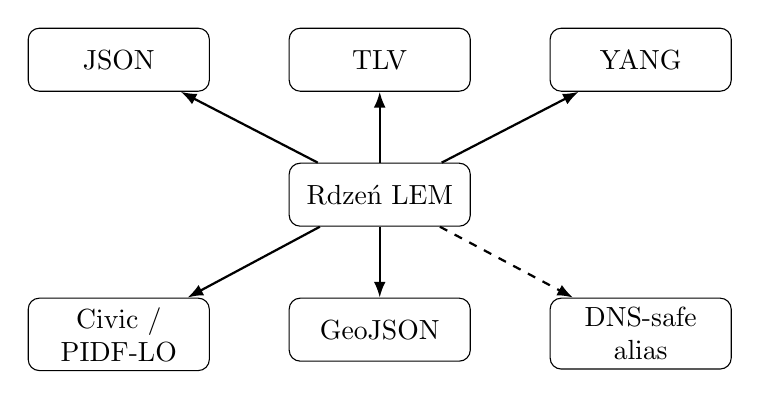
\begin{tikzpicture}[node distance=9mm and 10mm,
  box/.style={draw,rounded corners,align=center,minimum width=23mm,minimum height=8mm},
  arr/.style={-{Latex[length=2mm]},thick}]
  \node[box] (core) {Rdzeń LEM};
  \node[box,above left=of core] (json) {JSON};
  \node[box,above=of core] (tlv) {TLV};
  \node[box,above right=of core] (yang) {YANG};
  \node[box,below left=of core] (civic) {Civic /\\PIDF-LO};
  \node[box,below=of core] (geo) {GeoJSON};
  \node[box,below right=of core] (dns) {DNS-safe\\alias};
  \draw[arr] (core) -- (json);
  \draw[arr] (core) -- (tlv);
  \draw[arr] (core) -- (yang);
  \draw[arr] (core) -- (civic);
  \draw[arr] (core) -- (geo);
  \draw[arr,dashed] (core) -- (dns);
\end{tikzpicture}
\caption{Rdzeń semantyczny i jego reprezentacje oraz mapowania}
\label{fig:lem-representations}
\end{figure}

\section{Reprezentacja tekstowa (Human-readable)}
\label{sec:reprezentacja-tekstowa}
Reprezentacja tekstowa służy do czytelnego przedstawienia informacji o lokalizacji zdefiniowanej przez model LEM.

Reprezentacja tekstowa przedstawia komponenty modelu LEM w formie przeznaczonej do interpretacji przez człowieka. Sposób rozmieszczenia informacji, kolejność występowania komponentów, stosowane separatory lub formatowanie graficzne nie wpływają na znaczenie opisu informacji o lokalizacji.

Znaczenie reprezentacji tekstowej wynika wyłącznie z obecnych komponentów modelu LEM oraz ich interpretacji semantycznej.

\noindent \textbf{Przykład informacyjny:}
\begin{verbatim}
Site: Main Campus
Building: Engineering Center
Level: 2
Reference Space: Room 201
Relative Position: East side
\end{verbatim}

Powyższy zapis przedstawia informację o lokalizacji w sposób czytelny dla człowieka. Konkretna forma prezentacji nie stanowi części modelu semantycznego LEM.

\section{Reprezentacja binarna (Compact / TLV)}
\label{sec:reprezentacja-binarna}
Reprezentacja binarna umożliwia wyrażenie informacji LEM w postaci zwartej struktury danych przeznaczonej do wymiany lub przechowywania informacji.

Mechanizm kodowania binarnego nie definiuje znaczenia informacji o lokalizacji. Znaczenie każdego elementu reprezentacji wynika z odwzorowania na komponenty modelu LEM.

Reprezentacja binarna może wykorzystywać mechanizmy takie jak Type-Length-Value (TLV) --- wzorzec kodowania rozpoznawalny formalnie m.in. z rekomendacji ITU-T X.690 \cite{ITU-X690} (zob. Załącznik B) --- jednak sposób przypisania typów, kodowania wartości oraz organizacji struktury danych należy do określonej specyfikacji reprezentacji lub profilu implementacyjnego.

W reprezentacji binarnej:
\begin{itemize}
    \item typ elementu reprezentacji odpowiada komponentowi modelu LEM,
    \item wartość elementu reprezentacji odpowiada wartości określonego komponentu,
    \item sposób kodowania wartości nie zmienia znaczenia komponentu.
\end{itemize}

Poprawna reprezentacja binarna musi prowadzić do tej samej interpretacji semantycznej, jaka wynikaby z dowolnej innej poprawnej reprezentacji informacji LEM.

\noindent \textbf{Przykład informacyjny} (profil kodowania TLV zdefiniowany poniżej: T = 1 oktet, L = 2 oktety big-endian, V = wartość; \textit{Level} używa jednego oktetu \texttt{kind} oraz czterech oktetów \texttt{int32} dla wartości numerycznej):

\begin{verbatim}
Typ (T)  Nazwa komponentu     Długość (L)  Wartość (V)
0x01     Site                 0x000B       "Main Campus"
0x02     Building             0x0012       "Engineering Center"
0x03     Level                0x0005       0x01 00000002
0x04     Reference Space      0x0007       "Room201"
0x05     Relative Position    0x0009       "East side"
\end{verbatim}

\noindent \textbf{Ciąg oktetów (zapis szesnastkowy):}
\begin{verbatim}
01 00 0B 4D 61 69 6E 20 43 61 6D 70 75 73
02 00 12 45 6E 67 69 6E 65 65 72 69 6E 67 20 43 65 6E 74 65 72
03 00 05 01 00 00 00 02
04 00 07 52 6F 6F 6D 32 30 31
05 00 09 45 61 73 74 20 73 69 64 65
\end{verbatim}

Powyższe przypisanie wartości typu (T) do konkretnego komponentu (np. \texttt{0x03} $\rightarrow$ Level) jest elementem konkretnej specyfikacji reprezentacji lub profilu implementacyjnego, a nie częścią modelu semantycznego LEM --- inny profil binarny może przypisać te same komponenty do innych wartości T, pozostając równoważny semantycznie (zob. 2.4.3), o ile odwzorowanie na komponenty modelu jest jednoznaczne.

\subsection{Formalny rejestr typów (informacyjny)}
\label{sec:rejestr-typow}
Poniższy rejestr formalizuje powyższy przykład:
\begin{enumerate}
    \item Pole L ma 2 oktety, co pozwala opisać pełny zakres długości reprezentacji UTF-8.
    \item Kodowanie Level odzwierciedla strukturę kind+value i wspólną dziedzinę \texttt{int32}.
    \item Relative Position jest zwykłym ciągiem UTF-8, bez podtypu.
\end{enumerate}

\begin{table}[h]
\centering
\small
\begin{tabular}{|l|l|p{8cm}|}
\hline
\textbf{T (1 oktet)} & \textbf{Komponent} & \textbf{Kodowanie wartości (V)} \\ \hline
0x01 & Site & UTF-8 \cite{RFC3629}, 1--1024 oktetów; po dekodowaniu 1--256 punktów kodowych Unicode \\ \hline
0x02 & Building & UTF-8 \cite{RFC3629}, 1--1024 oktetów; po dekodowaniu 1--256 punktów kodowych Unicode \\ \hline
0x03 & Level & 1 oktet kind (0x01=numeric, 0x02=non-building) + dla numeric dokładnie 4 oktety liczby \texttt{int32} ze znakiem, uzupełnienie do dwóch, big-endian; dla non-building brak dalszych oktetów \\ \hline
0x04 & Reference Space & UTF-8 \cite{RFC3629}, 1--1024 oktetów; po dekodowaniu 1--256 punktów kodowych Unicode \\ \hline
0x05 & Relative Position & UTF-8 \cite{RFC3629}, 1--1024 oktetów; po dekodowaniu 1--256 punktów kodowych Unicode \\ \hline
\end{tabular}
\end{table}

\noindent \textbf{Format nagłówka:} T (1 oktet) + L (2 oktety, big-endian, długość V w oktetach) + V.\\
Reguły spójności 2.5.1–2.5.4 stosuje się do zbioru zdekodowanych komponentów dokładnie tak samo, jak w przypadku reprezentacji JSON (zob. 2.5.6).

\section{Reprezentacja JSON}
\label{sec:reprezentacja-json}
Reprezentacja JSON umożliwia wyrażenie informacji LEM przy użyciu struktury danych JSON. JSON stanowi wyłącznie sposób reprezentacji komponentów modelu LEM i nie definiuje własnej semantyki informacji o lokalizacji.

Reprezentacja używa JSON zgodnego z \cite{RFC8259}. Parser MUSI odrzucać obiekty zawierające zduplikowane nazwy właściwości rdzenia, zanim zostanie utworzona postać kanoniczna.

Struktura JSON musi umożliwiać jednoznaczne odwzorowanie elementów reprezentacji na komponenty modelu LEM.

Nazwy właściwości, struktura obiektu oraz sposób kodowania wartości są elementami reprezentacji i nie mogą zmieniać znaczenia komponentów zdefiniowanych w modelu LEM.

Dwa dokumenty JSON są semantycznie równoważne, jeżeli ich interpretacja prowadzi do tej samej interpretacji kanonicznej modelu LEM.

Różnice w:
\begin{itemize}[noitemsep,topsep=2pt]
    \item kolejności właściwości obiektu JSON,
    \item sposobie formatowania dokumentu,
    \item technicznej reprezentacji wartości, jeżeli zachowana jest równoważność znaczenia,
\end{itemize}
nie wpływają na równoważność semantyczną informacji.

\noindent \textbf{Przykład informacyjny:}
\begin{verbatim}
{
  "site": "Main Campus",
  "building": "Engineering Center",
  "level": { "kind": "numeric", "value": 2 },
  "referenceSpace": "Room201",
  "relativePosition": "East side"
}
\end{verbatim}

Poniższy dokument jest semantycznie równoważny powyższemu (inna kolejność właściwości, inne formatowanie):
\begin{verbatim}
{
  "level": { "value": 2, "kind": "numeric" },
  "site": "Main Campus",
  "relativePosition": "East side",
  "referenceSpace": "Room201",
  "building": "Engineering Center"
}
\end{verbatim}

Nazwy właściwości użyte powyżej (\texttt{site}, \texttt{building}, \texttt{level} itd.) są elementem konkretnej reprezentacji --- profil lub schemat implementacyjny MOŻE stosować inne nazwy (zob. 3.1, 4.4.4), o ile odwzorowanie na komponenty modelu LEM pozostaje jednoznaczne.

\noindent \textbf{Przykład informacyjny --- przypadek non-building} (zob. 2.1.6): obiekt znajdujący się na dachu budynku:
\begin{verbatim}
{
  "site": "Main Campus",
  "building": "Engineering Center",
  "level": { "kind": "non-building", "value": null },
  "referenceSpace": "Roof"
}
\end{verbatim}

\section{Alias prezentacyjny DNS-safe}
\label{sec:reprezentacja-dns-safe}
Alias DNS-safe umożliwia prezentację wybranego zakresu informacji LEM w środowiskach posiadających ograniczenia charakterystyczne dla nazw DNS \cite{RFC1035}.

Ograniczenia techniczne wynikające z zasad tworzenia nazw DNS nie definiują znaczenia informacji o lokalizacji.

Znaczenie reprezentacji DNS-safe wynika wyłącznie z odwzorowania użytych elementów na komponenty modelu LEM.

Alias DNS-safe może przedstawiać jedynie podzbiór komponentów modelu LEM. Brak możliwości wyrażenia określonego komponentu w danym środowisku nie zmienia znaczenia modelu, lecz oznacza utratę informacji w aliasie.

Zdefiniowana niżej kanonikalizacja tekstu jest stratna, dlatego DNS-safe \textbf{NIE JEST} równoważną ani odwracalną reprezentacją LEM. Jest wyłącznie aliasem prezentacyjnym. System wymagający odtworzenia postaci kanonicznej MUSI przenosić pełną reprezentację LEM innym kanałem lub stosować oddzielne, bezstratne kodowanie z jednoznacznym schematem dekodowania.

\noindent \textbf{Przykład informacyjny:}
\begin{verbatim}
level2.room201.eng-center.main-campus.loc.example.
\end{verbatim}

\subsection{Formalny schemat etykiet (informacyjny)}
\label{sec:schemat-etykiet}
Formalny schemat wprowadza jawne, krótkie prefiksy w każdej etykiecie, niezależne od jej pozycji w nazwie:

\begin{table}[h]
\centering
\small
\begin{tabular}{|l|l|p{7cm}|}
\hline
\textbf{Prefiks} & \textbf{Komponent} & \textbf{Kodowanie rdzenia etykiety} \\ \hline
s- & Site & Kanonikalizowany ciąg znaków \\ \hline
b- & Building & Kanonikalizowany ciąg znaków \\ \hline
l- & Level & \texttt{l-<N>} dla kind="numeric", wartość nieujemna; \texttt{l-n<N>} dla wartości ujemnej; \texttt{l-nb} dla kind="non-building" \\ \hline
r- & Reference Space & Kanonikalizowany ciąg znaków \\ \hline
\end{tabular}
\end{table}

\noindent Relative Position nigdy nie jest reprezentowany w DNS-safe.\\
Struktura pełnej nazwy (notacja ABNF, zgodnie z \cite{RFC5234}):
\begin{verbatim}
lem-dns-name  = *(component-label ".") suffix "."
component-label = prefix "-" label-core
prefix        = "s" / "b" / "l" / "r"
label-core    = 1*61(ALPHA / DIGIT / "-")
suffix        = 1*(dns-label ".") dns-label
\end{verbatim}

Kanonikalizacja wartości tekstowej (Site, Building, Reference Space) do rdzenia etykiety: zamiana na małe litery, zastąpienie spacji i innych znaków spoza \texttt{[a-z0-9]} znakiem \texttt{-}, zwinięcie kolejnych \texttt{-} do jednego, usunięcie \texttt{-} z brzegów. Ta kanonikalizacja jest stratna.

\noindent \textbf{Uwaga:} Punycode \cite{RFC3492} koduje Unicode w etykietach DNS, ale samo jego użycie nie odtwarza informacji utraconych przez usuwanie separatorów, zakres komponentów ani pominięcie \textit{Relative Position}. Bezstratny wariant wymaga osobnej specyfikacji.

\noindent \textbf{Przykład formalny:}
\begin{verbatim}
s-main-campus.b-engineering-center.l-2.r-room201.loc.example.
\end{verbatim}

\noindent \textbf{Przykład z Level ujemnym:}
\begin{verbatim}
s-main-campus.l-n1.r-parking-p1.loc.example.
\end{verbatim}

\noindent \textbf{Przykład z non-building (dach):}
\begin{verbatim}
s-main-campus.b-engineering-center.l-nb.r-roof.loc.example.
\end{verbatim}

\section{Mapowanie do istniejących modeli informacji}
\label{sec:mapowanie-modeli}
Istniejące modele informacji mogą być wykorzystywane do wyrażania wybranych aspektów informacji LEM poprzez zdefiniowane mapowania semantyczne.

Mapowanie do zewnętrznego modelu informacji nie oznacza zastąpienia modelu LEM ani rozszerzenia jego znaczenia.

Zewnętrzny model pełni rolę źródła reprezentacji określonych komponentów, których znaczenie musi być zgodne z interpretacją LEM.

Komponenty zewnętrznego modelu, które nie posiadają odpowiednika w modelu LEM, pozostają informacją dodatkową i nie stanowią części opisu informacji LEM.

\subsection{Mapowanie do modeli YANG}
\label{sec:mapowanie-yang}
Modele YANG mogą być wykorzystywane jako reprezentacja strukturalna komponentów LEM w środowiskach zarządzania sieciowego i systemowego.

\noindent \textbf{Przykład informacyjny --- poglądowy moduł YANG \cite{RFC7950}:}
\begin{verbatim}
module example-lem-location {
  namespace "urn:example:lem-location";
  prefix "lem";
  description
    "Poglądowe odwzorowanie komponentów modelu semantycznego LEM (Rozdział 2)
     na węzły danych YANG. Wyłącznie informacyjne (zob. 3.6.1).
     Struktura Level odzwierciedla 2.1.6 (kind/value).";

  grouping lem-location {
    description "Grupa węzłów odpowiadająca komponentom modelu LEM (zob. 2.1).";

    leaf site {
      type string { length "1..256"; }
      description "Odwzorowanie komponentu LEM: Site (zob. 2.1.6).";
    }

    leaf building {
      type string { length "1..256"; }
      description "Odwzorowanie komponentu LEM: Building (zob. 2.1.6).";
    }

    container level {
      description
        "Odwzorowanie komponentu LEM: Level (zob. 2.1.6). Struktura
         kind/value zamiast prostej liczby całkowitej.";

      leaf kind {
        type enumeration {
          enum numeric { description "Kondygnacja numerowana."; }
          enum non-building { description "Dach, parking naziemny, przestrzeń zewnętrzna itp."; }
        }
        mandatory true;
      }

      leaf value {
        type int32;
        when "../kind = 'numeric'";
        description "Wymagane i całkowite dla kind=numeric; nieobecne dla kind=non-building.";
      }

      must "(kind = 'numeric' and value) or (kind = 'non-building' and not(value))" {
        error-message "Zgodnie z 2.1.6: value wymagane dla kind=numeric, niedozwolone dla kind=non-building.";
      }
    }

    leaf reference-space {
      type string { length "1..256"; }
      description "Odwzorowanie komponentu LEM: Reference Space (zob. 2.1.6).";
    }

    leaf relative-position {
      type string { length "1..256"; }
      description "Odwzorowanie komponentu LEM: Relative Position (zob. 2.1.6) — opis relacyjny.";
      must "../reference-space" {
        error-message "Relative Position obecny bez Reference Space narusza LEM 2.5.3.";
      }
    }
  }

  container device-location {
    description "Przykładowy węzeł konfiguracyjny wykorzystujący grupę lem-location.";
    uses lem-location;
  }
}
\end{verbatim}

\subsection{Mapowanie do modeli Civic Address}
\label{sec:mapowanie-civic}
Modele Civic Address mogą być wykorzystywane do reprezentacji wybranych komponentów opisujących adresowe aspekty informacji o lokalizacji.

\noindent \textbf{Przykład informacyjny --- dokument PIDF-LO civicAddress \cite{RFC5139}:}
\begin{verbatim}
<civicAddress xml:lang="en-US"
 xmlns="urn:ietf:params:xml:ns:pidf:geopriv10:civicAddr">
  <country>US</country>
  <NAM>Main Campus</NAM>
  <BLD>Engineering Center</BLD>
  <FLR>2</FLR>
  <ROOM>Room201</ROOM>
  <LOC>East side</LOC>
</civicAddress>
\end{verbatim}

\begin{table}[h]
\centering
\small
\begin{tabularx}{\textwidth}{|>{\raggedright\arraybackslash}p{2.2cm}|>{\raggedright\arraybackslash}p{3.3cm}|>{\raggedright\arraybackslash}X|}
\hline
\textbf{CAtype} & \textbf{Komponent LEM} & \textbf{Charakter mapowania} \\ \hline
BLD (27) & Building & Odwzorowanie bezpośrednie. \\ \hline
FLR (28) & Level, kind="numeric" & Odwzorowanie dotyczy wyłącznie przypadku kind="numeric". \\ \hline
(brak wprost) & Level, kind="non-building" & Civic Address nie posiada elementu dedykowanego. \\ \hline
ROOM (23) & Reference Space & Odwzorowanie bezpośrednie. \\ \hline
NAM (22) & Site (interpretacja) & Interpretacyjne. \\ \hline
LOC (1) & Relative Position & Semantycznie bliskie, lecz nie identyczne. \\ \hline
\end{tabularx}
\caption{Mapowanie wybranych typów Civic Address \cite{RFC4776} na komponenty LEM}
\end{table}

\subsection{Mapowanie do modeli geospatial}
\label{sec:mapowanie-geospatial}
Modele geospatial mogą być wykorzystywane do wyrażania przestrzennych aspektów informacji o lokalizacji, w szczególności współrzędnych lub odniesień przestrzennych.

\noindent \textbf{Przykład informacyjny --- obiekt GeoJSON \cite{RFC7946}:}
\begin{verbatim}
{
  "type": "Feature",
  "geometry": {
    "type": "Point",
    "coordinates": [-73.961452, 40.808058]
  },
  "properties": {
    "lem:site": "Main Campus",
    "lem:building": "Engineering Center",
    "lem:level": { "kind": "numeric", "value": 2 },
    "lem:referenceSpace": "Room201",
    "lem:relativePosition": "East side"
  }
}
\end{verbatim}

\noindent Prefiks \texttt{lem:} w nazwach właściwości jest konwencją informacyjną. Kolejność współrzędnych \texttt{[longitude, latitude]} jest wymagana przez \cite{RFC7946} §4.

\section{Przykład ilustracyjny (jedna lokalizacja we wszystkich reprezentacjach)}
\label{sec:przyklad-ilustracyjny}
Poniższy przykład przedstawia tę samą informację o lokalizacji wyrażoną kolejno we wszystkich reprezentacjach. Wszystkie poniższe zapisy MUSZĄ prowadzić do tej samej interpretacji kanonicznej (zob. 2.4.5).

\noindent \textbf{Opisywana lokalizacja:} obiekt znajdujący się w budynku "Engineering Center" na kampusie "Main Campus", na drugiej kondygnacji, w pomieszczeniu "Room201", po wschodniej stronie tego pomieszczenia.

\begin{enumerate}
    \item \textbf{Reprezentacja tekstowa (3.2):}
\begin{verbatim}
Site: Main Campus
Building: Engineering Center
Level: 2 (numeric)
Reference Space: Room201
Relative Position: East side
\end{verbatim}

    \item \textbf{Reprezentacja binarna / TLV (3.3, wg formalnego rejestru 3.3.1 — pole L na 2 oktetach):}
\begin{verbatim}
01 00 0B 4D 61 69 6E 20 43 61 6D 70 75 73
02 00 12 45 6E 67 69 6E 65 65 72 69 6E 67 20 43 65 6E 74 65 72
03 00 05 01 00 00 00 02
04 00 07 52 6F 6F 6D 32 30 31
05 00 09 45 61 73 74 20 73 69 64 65
\end{verbatim}

    \item \textbf{Reprezentacja JSON (3.4):}
\begin{verbatim}
{
  "site": "Main Campus",
  "building": "Engineering Center",
  "level": { "kind": "numeric", "value": 2 },
  "referenceSpace": "Room201",
  "relativePosition": "East side"
}
\end{verbatim}

    \item \textbf{Alias prezentacyjny DNS-safe (3.5.1) --- zapis stratny:}
\begin{verbatim}
s-main-campus.b-engineering-center.l-2.r-room201.loc.example.
\end{verbatim}
\end{enumerate}

\section{Przykłady niepoprawnych opisów lokalizacji}
\label{sec:przyklady-niepoprawne}
\begin{itemize}
    \item \textbf{Przykład 1 --- naruszenie spójności relacji przestrzennych (2.5.3):}
\begin{verbatim}
{
  "site": "Main Campus",
  "building": "Engineering Center",
  "level": { "kind": "numeric", "value": 2 },
  "relativePosition": "East side"
}
\end{verbatim}
Obecny jest komponent \textit{Relative Position}, lecz brakuje \textit{Reference Space}.

    \item \textbf{Przykład 2 --- pusty opis lokalizacji (2.4.4):}
\begin{verbatim}
{}
\end{verbatim}

    \item \textbf{Przykład 3 --- naruszenie struktury Level (2.1.6):}
\begin{verbatim}
{
  "site": "Main Campus",
  "level": { "kind": "non-building", "value": 3 }
}
\end{verbatim}
\end{itemize}

% % =====================================================================
% Rozdział 4: Profile i zastosowania modelu LEM
% =====================================================================

\chapter{Profile i zastosowania modelu LEM}
\label{chap:profile}

\section{Rola profili LEM}
Profil LEM definiuje sposób zastosowania modelu LEM w określonym środowisku lub domenie.
Profil MOŻE ograniczać zakres wykorzystywanych komponentów oraz określać dodatkowe wymagania implementacyjne, lecz NIE ROZSZERZA modelu semantycznego LEM i NIE DEFINIUJE nowych komponentów informacji o lokalizacji.
Profil określa sposób wykorzystania istniejących komponentów modelu LEM w określonym kontekście zastosowania. Profil nie zmienia znaczenia komponentów modelu ani zasad ich interpretacji.

\section{Zasady definiowania profili}
Profil LEM MUSI spełniać następujące zasady:

\begin{itemize}
    \item \textbf{Zgodność semantyczna:} Profil NIE MOŻE zmieniać znaczenia komponentów modelu LEM ani definiować alternatywnej interpretacji informacji.
    \item \textbf{Ograniczenie zakresu:} Profil MOŻE ograniczać zakres wykorzystywanych komponentów, lecz NIE MOŻE usuwać ich znaczenia z modelu podstawowego.
    \item \textbf{Jednoznaczność wymagań:} Wymagania określone przez profil MUSZĄ wskazywać, które komponenty są wymagane, opcjonalne lub niewykorzystywane w danym zastosowaniu. Status obecności komponentu nie jest tożsamy z regułami obsługi nieznanych rozszerzeń z sekcji 7.7.
    \item \textbf{Niezależność reprezentacji:} Profil MOŻE określać wymagania dotyczące reprezentacji danych, lecz NIE MOŻE uzależniać znaczenia informacji od konkretnego formatu zapisu.
\end{itemize}

\section{Profile domenowe i przykłady zastosowań}
Poniższe podrozdziały opisują przykładowe domeny, w których model LEM może być stosowany. Każdy opis obejmuje zarówno rolę profilu danej domeny (co profil może ograniczać lub wymagać), jak i sposób integracji z systemami tej domeny — te dwa aspekty są ze sobą ściśle powiązane i celowo omawiane łącznie.

We wszystkich poniższych domenach obowiązuje wspólna zasada: integracja z systemem zewnętrznym NIE MOŻE zależeć od konkretnego protokołu, producenta ani technologii; informacja lokalizacyjna przekazywana pomiędzy systemami MUSI zachowywać znaczenie określone przez model semantyczny LEM; a ograniczenia techniczne systemu zewnętrznego nigdy nie stanowią rozszerzenia modelu LEM (zob. 3.1, 4.5). Jeżeli system zewnętrzny wymaga informacji nieposiadających odpowiednika w LEM, informacje te MUSZĄ być traktowane jako dane dodatkowe lub jako element profilu, zgodnie z zasadami niniejszego rozdziału.

\subsection{Infrastruktura sieciowa}
Profil infrastruktury sieciowej definiuje zastosowanie modelu LEM do opisu fizycznej lokalizacji elementów infrastruktury technicznej, takich jak punkty dostępowe, przełączniki, urządzenia IoT, systemy automatyki budynkowej oraz inne elementy wymagające jednoznacznej identyfikacji przestrzennej.

Integracja z systemami sieciowymi może obejmować urządzenia oraz systemy odpowiedzialne za obsługę infrastruktury technicznej — LEM pełni w tym przypadku rolę wspólnej warstwy semantycznej dla informacji o lokalizacji fizycznej urządzeń, natomiast NIE DEFINIUJE sposobu wykrywania urządzeń, zarządzania konfiguracją sieci ani mechanizmów komunikacji sieciowej.

Profil MOŻE określać wymagania dotyczące minimalnego zakresu informacji lokalizacyjnej wymaganej dla zarządzania infrastrukturą techniczną.

\subsection{Zarządzanie infrastrukturą i CMDB}
Profil zarządzania infrastrukturą i CMDB definiuje zastosowanie modelu LEM w systemach ewidencji, inwentaryzacji oraz dokumentacji technicznej zasobów — obejmując monitorowanie zasobów, zarządzanie konfiguracją, utrzymanie infrastruktury oraz automatyzację procesów operacyjnych.

System ewidencyjny MOŻE przechowywać informacje dodatkowe specyficzne dla własnej domeny, jednak informacje te NIE MOGĄ zmieniać interpretacji komponentów LEM. LEM NIE ZASTĘPUJE systemów zarządzania infrastrukturą — definiuje wyłącznie sposób jednoznacznego opisu znaczenia informacji lokalizacyjnej, umożliwiając interoperacyjność pomiędzy systemami o odmiennych strukturach danych.

\subsection{Lokalizacja awaryjna}
Profil usług lokalizacji awaryjnej definiuje zastosowanie modelu LEM w systemach wymagających przekazania informacji o lokalizacji dla celów bezpieczeństwa lub obsługi zdarzeń wymagających określenia fizycznego położenia.

LEM NIE DEFINIUJE usług ratunkowych, procedur bezpieczeństwa publicznego, mechanizmów obsługi zgłoszeń awaryjnych ani metod wyznaczania lokalizacji, i NIE ZASTĘPUJE istniejących standardów oraz systemów przeznaczonych do obsługi usług alarmowych. Rolą LEM jest reprezentacja oraz interpretacja informacji wynikowej dostarczonej przez system lokalizacyjny, zgodnie z zasadami modelu semantycznego określonymi w Rozdziale 2.

Profil MOŻE określać minimalny zakres informacji wymagany dla jednoznacznego określenia lokalizacji w danym środowisku. Ze względu na wagę tej domeny profil ten powinien szczególnie uwzględniać zasady dotyczące prywatności informacji lokalizacyjnej określone w sekcjach 6.3, 6.6 i 6.7.

\subsubsection{4.3.3.1. Przykładowe rozpisanie profilu (informacyjne)}
Poniżej przedstawiono jeden, w pełni rozpisany przykład profilu „Lokalizacja awaryjna” — od wymagań, przez formalny schemat, po przetestowane przykłady zgodne i niezgodne. Ma to charakter wyłącznie ilustracyjny; rzeczywisty profil dla konkretnego wdrożenia powinien zostać ustalony przez podmiot odpowiedzialny za dane środowisko (zob. 4.1).

Wymagania komponentów (zgodnie z zasadą „Jednoznaczność wymagań”, 4.2):

\begin{table}[htbp]
\centering
\begin{tabular}{|l|l|p{7cm}|}
\hline
\textbf{Komponent} & \textbf{Status w profilu} & \textbf{Uzasadnienie} \\ \hline
Building & Wymagany & Zespół ratunkowy musi wiedzieć, do którego budynku się udać. \\ \hline
Level & Wymagany & Kondygnacja jest krytyczna dla nawigacji w budynkach wielopiętrowych. \\ \hline
Reference Space & Wymagany & Pomieszczenie/przestrzeń referencyjna jest minimalną jednostką lokalizacji użyteczną operacyjnie. \\ \hline
Site & Opcjonalny & Istotny wyłącznie w organizacjach wielokampusowych; jeśli obecny, zwiększa jednoznaczność. \\ \hline
Relative Position & Opcjonalny (zalecany) & Zwiększa precyzję w obrębie Reference Space, lecz nie jest niezbędny do podjęcia interwencji. \\ \hline
\end{tabular}
\caption{Wymagania komponentów dla profilu lokalizacji awaryjnej}
\label{tab:emergency_profile}
\end{table}

Statusy w tabeli określają kompletność danych wymaganą przez profil. Nie określają sposobu obsługi nieznanych rozszerzeń reprezentacji.

Formalny schemat (JSON Schema, informacyjny), rozszerzający szkielet strukturalny modelu podstawowego (2.5.6) przez \texttt{allOf}:

\begin{verbatim}
{
  "$schema": "https://json-schema.org/draft/2020-12/schema",
  "$id": "https://w3id.org/lem/1.0/profile/emergency",
  "title": "LEM — profil: Lokalizacja awaryjna (zob. 4.3.3)",
  "allOf": [
    { "$ref": "https://w3id.org/lem/1.0/schema/core" }
  ],
  "required": [
    "building",
    "level",
    "referenceSpace"
  ]
}
\end{verbatim}

Przykład zgodny z profilem:
\begin{verbatim}
{
  "site": "Main Campus",
  "building": "Engineering Center",
  "level": {
    "kind": "numeric",
    "value": 2
  },
  "referenceSpace": "Room201",
  "relativePosition": "East side, near window"
}
\end{verbatim}

Przykład niezgodny z profilem (lecz zgodny z modelem podstawowym LEM):
\begin{verbatim}
{
  "site": "Main Campus",
  "building": "Engineering Center"
}
\end{verbatim}

\textbf{Uwaga dot. weryfikacji.} Powyższy przykład „niezgodny” został celowo tak dobrany, aby zaprezentować regułę z sekcji 4.4.3: zweryfikowany względem szkieletu modelu podstawowego (2.5.6) dokument ten dał wynik POPRAWNE — to w pełni ważny opis LEM (opis częściowy, zob. 2.4.4). Ten sam dokument zweryfikowany względem schematu profilu dał wynik NIEPOPRAWNE, z dwoma konkretnymi błędami: brakiem pól \texttt{level} i \texttt{referenceSpace}. Jest to bezpośrednie potwierdzenie zasady 4.4.3: „Informacja może być poprawną reprezentacją LEM, lecz jednocześnie nie spełniać wymagań konkretnego profilu zastosowania.”

\subsection{Systemy indoor positioning}
Profil systemów indoor positioning definiuje zastosowanie modelu LEM w środowiskach lokalizacji wewnętrznej, w których położenie określane jest względem przestrzeni referencyjnych oraz relacji przestrzennych.

Profil NIE DEFINIUJE technologii wyznaczania pozycji ani metod pomiarowych. Określa wyłącznie sposób wyrażenia informacji lokalizacyjnej zgodnie z modelem LEM. LEM NIE DEFINIUJE metod pomiaru ani algorytmów lokalizacyjnych wykorzystywanych przez systemy dostarczające dane wejściowe.

\subsection{Dokumentacja techniczna}
LEM MOŻE być wykorzystywany do tworzenia spójnych opisów lokalizacji elementów infrastruktury w dokumentacji technicznej, systemach ewidencyjnych oraz narzędziach wspierających utrzymanie infrastruktury.

Informacja zgodna z LEM MOŻE być przechowywana lub prezentowana w różnych systemach dokumentacyjnych przy zachowaniu tej samej interpretacji semantycznej. LEM NIE DEFINIUJE formatów dokumentacji, narzędzi dokumentacyjnych, metod tworzenia dokumentacji ani procesów zarządzania zmianą dokumentacji technicznej.

\subsection{Automatyzacja i orkiestracja}
LEM MOŻE być wykorzystywany jako warstwa semantyczna dla systemów automatyzacji i orkiestracji wymagających dostępu do informacji o lokalizacji elementów infrastruktury. Informacja lokalizacyjna zgodna z LEM MOŻE być wykorzystywana przez systemy zewnętrzne jako dane wejściowe do realizacji procesów automatycznych.

LEM NIE DEFINIUJE mechanizmów automatyzacji, reguł sterowania, logiki orkiestracji ani sposobów wykorzystania informacji lokalizacyjnej przez systemy wykonawcze.

\subsection{Inne domeny}
Model LEM MOŻE być stosowany w innych domenach wymagających jednoznacznej reprezentacji lub wymiany informacji o lokalizacji (np. systemy automatyki budynkowej, systemy bezpieczeństwa, systemy dokumentacji przestrzennej, systemy analityczne, systemy orkiestracji zasobów), jeżeli sposób wykorzystania modelu zachowuje zgodność z zasadami określonymi w niniejszej specyfikacji.

Nowe zastosowania NIE MOGĄ zmieniać znaczenia komponentów modelu LEM ani definiować alternatywnej interpretacji informacji lokalizacyjnej. Wymagania specyficzne dla określonej domeny POWINNY być definiowane poprzez profile LEM zgodnie z zasadami niniejszego rozdziału.

\section{Ograniczenia i wymagania implementacyjne profili}
Profile mogą określać wymagania implementacyjne wynikające ze specyfiki określonej domeny zastosowania. Wymagania te dotyczą sposobu wykorzystania modelu LEM i NIE STANOWIĄ rozszerzenia jego podstawowej semantyki.

\subsection{Minimalny zakres informacji}
Profil MOŻE określać minimalny zestaw komponentów wymaganych do obsługi informacji o lokalizacji zgodnie z danym zastosowaniem. Minimalny zakres informacji określony przez profil NIE ZMIENIA znaczenia komponentów modelu LEM.

\subsection{Wymagane komponenty}
Profil MOŻE określać komponenty modelu, których obecność jest wymagana w określonym zastosowaniu. Wymaganie obecności komponentu wynika z potrzeb konkretnego profilu i NIE OZNACZA, że komponent ten jest obowiązkowy w podstawowym modelu LEM.

\subsection{Reguły walidacji profilu}
Walidacja profilu jest procesem weryfikacji zgodności opisu lokalizacji z wymaganiami określonymi przez dany profil.

Walidacja profilu jest niezależna od podstawowej interpretacji semantycznej modelu LEM. Informacja może być poprawną reprezentacją LEM, lecz jednocześnie nie spełniać wymagań konkretnego profilu zastosowania.

\subsection{Specyficzne schematy danych}
Profile MOGĄ definiować techniczne schematy danych, takie jak JSON Schema, typy pól, ograniczenia wartości, reguły walidacyjne oraz wymagania implementacyjne.

Schematy te określają sposób wykorzystania modelu LEM w konkretnym środowisku i NIE STANOWIĄ rozszerzenia modelu semantycznego LEM.

Poniższy szkielet JSON Schema ma charakter wyłącznie informacyjny i ilustruje, jak profil może formalnie wyrazić wymagania określone prozą w sekcjach 4.4.1–4.4.2:

\begin{verbatim}
{
  "$schema": "https://json-schema.org/draft/2020-12/schema",
  "$id": "https://w3id.org/lem/1.0/profile/network-infrastructure",
  "title": "Przykładowy profil: infrastruktura sieciowa",
  "allOf": [
    { "$ref": "https://w3id.org/lem/1.0/schema/core" },
    {
      "type": "object",
      "required": ["building", "referenceSpace"],
      "not": { "required": ["relativePosition"] }
    }
  ]
}
\end{verbatim}

Zgodność danych z powyższym schematem stanowi walidację zgodności z profilem (zob. 4.4.3, 5.3) i jest niezależna od walidacji podstawowej zgodności semantycznej z modelem LEM określonej w sekcji 2.5.

\section{Zgodność profili z modelem LEM}
Każdy profil MUSI zachować zgodność z modelem semantycznym LEM określonym w Rozdziale 2.

Profil NIE MOŻE:
\begin{itemize}
    \item zmieniać interpretacji komponentów modelu,
    \item definiować alternatywnej semantyki informacji o lokalizacji,
    \item wprowadzać nowych komponentów semantycznych,
    \item traktować ograniczeń technicznych systemu zewnętrznego jako podstawy do rozszerzenia modelu LEM.
\end{itemize}

Zgodność z LEM jest niezależna od zgodności z wymaganiami konkretnego profilu. System MOŻE być poprawną reprezentacją informacji LEM, nawet jeżeli NIE REALIZUJE wymagań określonego profilu zastosowania.

\section{Rozszerzanie i wersjonowanie profili}
Profile LEM mogą ewoluować w czasie w odpowiedzi na zmieniające się wymagania domenowe. Ewolucja profili NIE MOŻE naruszać stabilności semantycznej podstawowego modelu LEM. Ogólne zasady klasyfikacji zmian modelu (korekcyjna / rozszerzająca / semantyczna) określone w Rozdziale 7 stosuje się odpowiednio do ewolucji profili.

\subsection{Dziedziczenie profili}
Profile MOGĄ tworzyć specjalizacje istniejących profili. Profil potomny MOŻE rozszerzać wymagania profilu nadrzędnego, lecz NIE MOŻE: zmieniać znaczenia komponentów odziedziczonych, usuwać interpretacji określonych przez profil nadrzędny, ani naruszać ograniczeń wynikających z profilu nadrzędnego.

\subsection{Kompatybilność wsteczna}
Ewolucja profilu NIE MOŻE prowadzić do zmiany interpretacji komponentów używanych w starszych wersjach profilu. Zmiany profilu powinny umożliwiać zachowanie zgodności istniejących implementacji wszędzie tam, gdzie nie zmienia się podstawowa semantyka modelu LEM.

\subsection{Ewolucja profili domenowych}
Profile domenowe MOGĄ być aktualizowane w odpowiedzi na zmieniające się potrzeby środowisk zastosowania. Aktualizacja profilu MUSI zachować: zgodność z modelem semantycznym LEM, stabilność interpretacji istniejących komponentów oraz możliwość jednoznacznego określenia różnic pomiędzy wersjami profilu.

Ewolucja profili NIE MOŻE wymagać zmian w podstawowym modelu semantycznym LEM, jeżeli potrzeba zmiany wynika wyłącznie z wymagań konkretnej domeny zastosowania.


% % --- Bibliografia ---------------------------------------------------
% % Dokument zrodlowy nie zawiera cytowan - sekcja przygotowana do
% % wlaczenia po dodaniu pozycji do bibliography.bib i wstawieniu \cite{}.
% % \bibliographystyle{plalpha}
% % {\raggedright\sloppy\small\bibliography{bibliography}}

% \end{document}

% =====================================================================
% TREŚĆ
% =====================================================================
\mainmatter
\renewcommand{\thefigure}{\thechapter.\arabic{figure}.}
\renewcommand{\thetable}{\thechapter.\arabic{table}.}

% =====================================================================
% Rozdzial 1: Wprowadzenie
% =====================================================================

\chapter{Wprowadzenie}
\label{chap:wprowadzenie}

\section{Cel modelu LEM}
\label{sec:cel-lem}
Informacja o lokalizacji jest wykorzystywana przez wiele systemów technicznych działających w różnych domenach zastosowań. Systemy zarządzania infrastrukturą, automatyzacji, bezpieczeństwa, dokumentacji technicznej oraz usług lokalizacyjnych wymagają jednoznacznego opisu położenia obiektów fizycznych. W praktyce informacje te są często reprezentowane przy użyciu lokalnych konwencji zależnych od systemu, producenta lub technologii. Stosowane podejścia obejmują między innymi:

\begin{itemize}
    \item nieustrukturyzowane opisy tekstowe w systemach CMDB, bazach danych lub dokumentacji technicznej,
    \item lokalne schematy nazewnictwa urządzeń i przestrzeni,
    \item oznaczenia wynikające z dokumentacji architektonicznej lub organizacyjnej,
    \item informacje utrzymywane jako wiedza operacyjna określonych osób lub zespołów.
\end{itemize}

Takie sposoby opisu często nie zapewniają jednoznacznej, deterministycznej i maszynowo interpretowalnej informacji. Konsekwencją braku wspólnego modelu semantycznego są m.in. ograniczona interoperacyjność, utrudniona automatyzacja oraz problemy z utrzymaniem spójności.

Model Kodowania Lokalizacji (\textit{Location Encoding Model}, LEM) definiuje wspólny model semantyczny, którego celem jest zapewnienie jednoznacznego znaczenia komponentów niezależnie od sposobu ich reprezentacji czy implementacji. LEM definiuje znaczenie informacji, podczas gdy sposób jej wyrażenia w konkretnym formacie pozostaje warstwą niezależną.

\section{Zakres dokumentu}
\label{sec:zakres}
Niniejszy dokument definiuje \textit{Location Encoding Model} (LEM) jako model informacji przeznaczony do opisu lokalizacji. Specyfikacja określa:

\begin{itemize}
    \item model semantyczny informacji o lokalizacji,
    \item komponenty modelu LEM oraz ich znaczenie,
    \item zasady interpretacji informacji, równoważności semantycznej oraz spójności modelu,
    \item zasady reprezentacji informacji LEM oraz tworzenia profili zastosowań.
\end{itemize}

Dokument nie definiuje formatów wymiany danych, protokołów komunikacyjnych, technologii pomiaru lokalizacji, algorytmów pozycjonowania ani wymagań specyficznych dla pojedynczego środowiska.

LEM nie definiuje mechanizmów identyfikacji obiektów, pozyskiwania informacji lokalizacyjnej ani metod określania położenia. Model opisuje wyłącznie semantykę informacji o lokalizacji już dostępnej.

\section{Wkład dokumentu}
\label{sec:wklad}
Wkład LEM obejmuje cztery elementy:
\begin{enumerate}
    \item niewielki rdzeń semantyczny oddzielający znaczenie lokalizacji od jej reprezentacji;
    \item deterministyczną postać kanoniczną i jawne reguły równoważności opisów częściowych;
    \item spójne odwzorowania na JSON, TLV i YANG oraz mapowania integracyjne do Civic Address i GeoJSON;
    \item mechanizm profili umożliwiający specjalizację domenową bez redefiniowania rdzenia modelu.
\end{enumerate}

\section{Niezależność semantyki od reprezentacji}
\label{sec:niezaleznosc}
Model LEM rozdziela znaczenie informacji od sposobu jej wyrażenia. Znaczenie jest określone przez model semantyczny i interpretację kanoniczną. Ta sama informacja może być wyrażona w różnych reprezentacjach (tekstowej, strukturalnej, binarnej), które są semantycznie równoważne, jeśli prowadzą do tej samej interpretacji zgodnie z zasadami LEM.

\section{Struktura dokumentu}
\label{sec:struktura-dok}
\begin{description}
    \item[Rozdział 2:] Definiuje model semantyczny LEM, komponenty oraz zasady interpretacji.
    \item[Rozdział 3:] Definiuje zasady reprezentacji modelu w różnych formatach danych.
    \item[Rozdział 4:] Definiuje profile zastosowań dla specjalizacji domenowych.
    \item[Rozdziały 5--7:] Omawiają implementację, bezpieczeństwo, prywatność i ewolucję modelu.
    \item[Rozdział 8:] Osadza LEM względem istniejących standardów i modeli.
\end{description}

\section{Terminologia i konwencje}
\label{sec:terminologia}
Na potrzeby dokumentu przyjęto następujące definicje:

\begin{description}
    \item[Model informacji (\textit{Information Model}):] Abstrakcyjny model definiujący strukturę, znaczenie oraz relacje elementów.
    \item[Informacja o lokalizacji:] (\textit{Location Information}) Informacja opisana przy użyciu komponentów LEM.
    \item[Komponent modelu (\textit{Model Component}):] Element LEM posiadający znaczenie semantyczne.
    \item[Przestrzeń referencyjna (\textit{Reference Space}):] Przestrzeń odniesienia dla interpretacji przestrzennej.
    \item[Położenie względne (\textit{Relative Position}):] Relacja przestrzenna względem przestrzeni referencyjnej.
    \item[Reprezentacja (\textit{Representation}):] Sposób wyrażenia informacji przy użyciu formatu danych.
    \item[Interpretacja kanoniczna (\textit{Canonical Interpretation}):] Jednoznaczne znaczenie wynikające z modelu LEM.
    \item[Profil LEM (\textit{LEM Profile}):] Specjalizacja modelu określająca wymagania dla danego zastosowania.
\end{description}

Słowa kluczowe zapisane wielkimi literami są używane zgodnie z BCP~14 \cite{RFC2119,RFC8174}: \textbf{MUSI} odpowiada \textit{MUST}, \textbf{NIE MOŻE} --- \textit{MUST NOT}, \textbf{POWINIEN} --- \textit{SHOULD}, a \textbf{MOŻE} --- \textit{MAY}. Przykłady mają charakter ilustracyjny, o ile nie oznaczono ich inaczej.

% =====================================================================
% Rozdział 2: Model semantyczny LEM
% =====================================================================

\chapter{Model semantyczny LEM}
\label{chap:model}

\section{Komponenty modelu}
\label{sec:komponenty}
\textit{Location} jest logiczną kompozycją komponentów semantycznych opisujących fizyczną lokalizację obiektu. Poszczególne komponenty dostarczają informacji o różnych aspektach lokalizacji i mogą występować niezależnie od siebie, z uwzględnieniem ograniczeń określonych w niniejszej specyfikacji.

Model LEM definiuje zestaw komponentów semantycznych służących do opisu fizycznej lokalizacji obiektu. Każdy komponent reprezentuje określony aspekt informacji lokalizacyjnej i posiada niezależną semantykę. Komponenty mogą być stosowane pojedynczo lub łączone w celu uzyskania większego poziomu szczegółowości opisu lokalizacji.

\begin{figure}[htbp]
\centering
\begin{tikzpicture}[node distance=9mm and 8mm,
  box/.style={draw,rounded corners,align=center,minimum width=25mm,minimum height=8mm},
  arr/.style={-{Latex[length=2mm]},thick}]
  \node[box] (entity) {Encja};
  \node[box,right=of entity] (location) {Location};
  \node[box,below left=of location] (site) {Site};
  \node[box,below=of location] (building) {Building};
  \node[box,below right=of location] (level) {Level};
  \node[box,below=18mm of site] (ref) {Reference\\Space};
  \node[box,below=18mm of level] (rel) {Relative\\Position};
  \draw[arr] (entity) -- (location);
  \draw[arr] (location) -- (site);
  \draw[arr] (location) -- (building);
  \draw[arr] (location) -- (level);
  \draw[arr] (location) -- (ref);
  \draw[arr] (location) -- (rel);
  \draw[arr,dashed] (rel) -- node[below,sloped,font=\scriptsize]{względem} (ref);
\end{tikzpicture}
\caption{Rdzeń semantyczny modelu LEM}
\label{fig:lem-core}
\end{figure}

O ile niniejsza specyfikacja nie określa inaczej, brak komponentu oznacza brak określonej informacji, a nie wartość domyślną (zob. sekcja \ref{sec:opisy-czesciowe}).

Poniższe sekcje definiują znaczenie poszczególnych komponentów oraz podstawowe reguły ich wykorzystania. Zasady dotyczące zależności pomiędzy komponentami, wymagań minimalnych, walidacji semantycznej, przypadków niepełnej lokalizacji oraz konfliktu informacji są określone łącznie w sekcjach \ref{sec:kanoniczna-interpretacja} (Kanoniczna interpretacja) oraz \ref{sec:spojnosci-modelu} (Reguły spójności modelu).

\subsection{Site}
\label{sec:comp-site}
\textit{Site} --- najwyższy poziom hierarchii lokalizacji, definiowany przez implementację.

\subsection{Building}
\label{sec:comp-building}
\textit{Building} --- element hierarchii lokalizacji reprezentujący pojedynczy budynek lub inny wydzielony obiekt przestrzenny, definiowany przez implementację.

\subsection{Level}
\label{sec:comp-level}
\textit{Level} --- element hierarchii lokalizacji reprezentujący poziom przestrzeni, definiowany przez implementację.

\subsection{Reference Space}
\label{sec:comp-refspace}
\textit{Reference Space} --- jednoznacznie identyfikowalna przestrzeń stanowiąca punkt odniesienia do określenia położenia względnego obiektu.

\subsection{Relative Position}
\label{sec:comp-relpos}
\textit{Relative Position} --- opis położenia obiektu względem zdefiniowanej przestrzeni referencyjnej.

Znaczenie każdego komponentu oraz relacji pomiędzy nimi jest niezależne od reprezentacji, w której komponent został zapisany (zob. Rozdział 3).

\subsection{Formalne typy danych komponentów (normatywne)}
\label{sec:typy-danych}
Lokalizacja encji jest reprezentowana przez pięć niezależnych komponentów. Każdy komponent ma zdefiniowany typ i semantykę. Wartości tekstowe zawierają od 1 do 256 punktów kodowych Unicode. UTF-8 \cite{RFC3629} jest kodowaniem stosowanym przez wybrane reprezentacje, a nie miarą długości semantycznej.

\begin{description}
    \item[Site:]
    \begin{itemize}
        \item \textbf{Typ:} \texttt{string}
        \item \textbf{Semantyka:} nazwa lub identyfikator tekstowy miejsca/siedziby/kampusu, w obrębie którego znajduje się \textit{Building}.
        \item \textbf{Wymaganie:} komponent opcjonalny w modelu podstawowym; profil może wymagać jego obecności.
        \item \textbf{Uwaga projektowa (nie stanowi części modelu):} w przyszłych integracjach z systemami zewnętrznymi (CMDB, GIS) zaleca się rozróżnienie wartości prezentacyjnej (\texttt{name}) od stabilnego identyfikatora. Obecny model tego rozróżnienia nie wprowadza.
    \end{itemize}

    \item[Building:]
    \begin{itemize}
        \item \textbf{Typ:} \texttt{string}
        \item \textbf{Semantyka:} nazwa lub identyfikator tekstowy budynku (lub równoważnego obiektu budowlanego) znajdującego się w \textit{Site}.
        \item \textbf{Wymaganie:} komponent opcjonalny w modelu podstawowym.
        \item \textbf{Uwaga projektowa:} analogicznie do \textit{Site}.
    \end{itemize}

    \item[Level:]
    \begin{itemize}
        \item \textbf{Typ:} struktura \texttt{Level} z polami \texttt{kind} oraz \texttt{value}.
        \item \textbf{Semantyka:} 
        \begin{itemize}
            \item \texttt{kind = "numeric"} --- \texttt{value} jest wymagane i musi być liczbą całkowitą ze znakiem w zakresie od $-2^{31}$ do $2^{31}-1$. \texttt{0} oznacza poziom parteru / ground floor (konwencja modelu, niezależna od lokalnej numeracji źródłowej). Wartości dodatnie oznaczają kondygnacje nadziemne; wartości ujemne oznaczają kondygnacje podziemne.
            \item \texttt{kind = "non-building"} --- \texttt{value} musi być \texttt{null}. Oznacza, że encja nie znajduje się na żadnej kondygnacji budynku (dach, parking naziemny, przestrzeń zewnętrzna, strefa pomiędzy budynkami itp.). Przestrzeń taka jest w takim wypadku dalej opisywana przez \textit{Reference Space} (np. \texttt{"Roof"}), a nie przez \texttt{value}.
        \end{itemize}
        \item \textbf{Wymaganie:} komponent opcjonalny w modelu podstawowym.
        \item \textbf{Zakaz:} wartości ułamkowe oraz inne typy niż określone powyżej są niedozwolone. Przypadek antresoli pozostaje nieobsłużony przez model podstawowy.
    \end{itemize}

    \item[Reference Space:]
    \begin{itemize}
        \item \textbf{Typ:} \texttt{string}
        \item \textbf{Semantyka:} nazwana lub w inny sposób określona przestrzeń stanowiąca kontekst lokalizacyjny dla encji --- pomieszczenie, sala, pokój, korytarz, hala, parking, dach, strefa zewnętrzna lub inna przestrzennie znacząca jednostka. \textit{Reference Space} nie jest ograniczony do pojęcia „pomieszczenie”.
        \item \textbf{Wymaganie:} komponent opcjonalny. Pusty ciąg jest niedozwolony; brak informacji wyraża się nieobecnością komponentu.
    \end{itemize}

    \item[Relative Position:]
    \begin{itemize}
        \item \textbf{Typ:} \texttt{string}
        \item \textbf{Semantyka:} opis pozycji encji względem \textit{Reference Space} (np. \texttt{"przy oknie"}, \texttt{"wschodnia ściana"}, \texttt{"nad szafą R1"}, \texttt{"centralnie"}, \texttt{"przy wejściu"}). Wartość jest opisem relacyjnym --- model nie wymaga ani nie narzuca reprezentacji współrzędnych.
        \item \textbf{Wymaganie:} pole opcjonalne. Zgodnie z sekcją \ref{sec:spojnosc-przestrzenna}, jeżeli obecne, wymaga obecności \textit{Reference Space} w tym samym opisie.
    \end{itemize}
\end{description}

\noindent \textbf{Wspólne reguły:}
\begin{itemize}
    \item Wszystkie wartości tekstowe mają długość od 1 do 256 punktów kodowych Unicode. Limit liczby oktetów jest właściwością reprezentacji.
    \item Poprawny opis zawiera co najmniej jeden komponent rdzenia.
    \item Komponenty są niezależne --- brak wartości w jednym polu nie unieważnia pozostałych (zob. sekcja \ref{sec:opisy-czesciowe}).
    \item Model nie definiuje hierarchii referencyjnej (encje Site/Building jako obiekty odrębne od swoich wartości tekstowych). Komponenty pełnią wyłącznie rolę lokalizacyjną.
\end{itemize}

\section{Relacje pomiędzy komponentami}
\label{sec:relacje}
Komponenty modelu LEM są powiązane relacjami (zob. Appendix A.6). Relacje w modelu LEM są kierunkowe (zob. Appendix A.13) --- kolejność elementów uczestniczących w relacji stanowi część jej znaczenia semantycznego i nie może być pomijana podczas interpretacji.

Przykładowo, relacja \texttt{located\_in(Object, ReferenceSpace)} posiada inne znaczenie niż relacja odwrotna \texttt{contains(ReferenceSpace, Object)}. Zachowanie kierunku relacji jest warunkiem poprawnej interpretacji opisu lokalizacji zgodnie z zasadami określonymi w sekcji \ref{sec:spojnosc-przestrzenna}.

\section{Klasyfikacja przestrzeni referencyjnych}
\label{sec:klasyfikacja-przestrzeni}
Przestrzeń referencyjna określa rodzaj przestrzeni wykorzystywanej jako odniesienie dla opisu relacji przestrzennej w modelu LEM.

Klasyfikacja przestrzeni referencyjnych służy organizacji możliwych kategorii odniesienia i nie definiuje zamkniętego zbioru typów przestrzeni. LEM nie określa wyczerpującej listy klas przestrzeni referencyjnych. Implementacje mogą definiować dodatkowe klasy zgodnie z wymaganiami określonego zastosowania, o ile zachowana zostaje semantyka modelu LEM.

Klasyfikacja przestrzeni referencyjnych nie wpływa na znaczenie informacji o lokalizacji. Znaczenie opisu informacji o lokalizacji wynika z interpretacji komponentów modelu LEM oraz relacji pomiędzy nimi zgodnie z zasadami określonymi w sekcji \ref{sec:kanoniczna-interpretacja}.

Przynależność przestrzeni referencyjnej do określonej klasy nie zmienia sposobu interpretacji relacji \textit{Relative Position}, o której mowa w sekcji \ref{sec:spojnosc-przestrzenna} --- klasyfikacja ma charakter porządkujący, a nie znaczeniowy.

\section{Kanoniczna interpretacja}
\label{sec:kanoniczna-interpretacja}
Kanoniczna interpretacja definiuje deterministyczną postać opisu po zdekodowaniu reprezentacji. Nie rozstrzyga, czy różne nazwy naturalnojęzykowe oznaczają ten sam obiekt.

\subsection{Cel interpretacji kanonicznej}
\label{sec:cel-interpretacji}
Kanoniczna interpretacja umożliwia porównanie poprawnych reprezentacji bez zależności od kolejności pól, formatowania lub technologii transportu.

\subsection{Interpretacja opisu informacji}
\label{sec:interpretacja-opisu}
Po poprawnym zdekodowaniu opisu $D$ jego postać kanoniczna jest uporządkowaną krotką częściową
\[
C(D)=(S?,B?,L?,R?,P?),
\]
gdzie symbole odpowiadają kolejno komponentom \textit{Site}, \textit{Building}, \textit{Level}, \textit{Reference Space} i \textit{Relative Position}, a znak zapytania oznacza możliwość nieobecności wartości. Nieobecność nie jest wartością pustą ani domyślną.

Wartości tekstowe w $C(D)$ są dokładnymi ciągami Unicode dostarczonymi przez reprezentację. Model podstawowy nie wykonuje automatycznego przycinania białych znaków, zmiany wielkości liter, tłumaczenia, rozwijania skrótów ani rozpoznawania synonimów. Profil może zdefiniować jawne reguły normalizacji lub stabilne identyfikatory, ale muszą one poprzedzać utworzenie $C(D)$ i być identycznie stosowane przez porównywane implementacje.

\subsection{Równoważność semantyczna}
\label{sec:rownowaznosc-semantyczna}
Dwa poprawne opisy $D_1$ i $D_2$ są równoważne w modelu podstawowym wtedy i tylko wtedy, gdy $C(D_1)=C(D_2)$, tj. zawierają dokładnie ten sam podzbiór komponentów i identyczne wartości po zdekodowaniu.

Na równoważność semantyczną nie wpływają:
\begin{itemize}[noitemsep,topsep=2pt]
    \item kolejność występowania komponentów w opisie informacji o lokalizacji,
    \item sposób reprezentacji informacji,
    \item format zapisu informacji,
    \item obecność dodatkowych informacji niezdefiniowanych przez model LEM, o ile są oddzielone od komponentów rdzenia i nie wpływają na ich dekodowanie.
\end{itemize}

\subsection{Opisy częściowe}
\label{sec:opisy-czesciowe}
Opis informacji o lokalizacji może zawierać dowolny niepusty podzbiór komponentów zdefiniowanych przez model LEM, z zastrzeżeniem, że \textit{Relative Position} wymaga obecności \textit{Reference Space}.

Brak komponentu oznacza brak określonej informacji w danym zakresie i nie stanowi naruszenia modelu LEM.

Opis częściowy reprezentuje mniejszy zakres informacji o lokalizacji niż opis zawierający dodatkowe komponenty, lecz pozostaje poprawnym opisem semantycznym.

Wymagania dotyczące minimalnego zakresu informacji dla określonych zastosowań mogą być definiowane poza modelem LEM --- w szczególności poprzez profile zastosowań (Rozdział 4).

\noindent \textbf{Uwaga dot. prywatności:} Nawet opis częściowy, ograniczony do niewielkiej liczby komponentów, może w określonym kontekście stanowić informację wystarczającą do pośredniej identyfikacji osoby lub zasobu. Model LEM pozostaje neutralny wobec tej oceny (zob. sekcja 6.6), lecz profile zastosowań powinny brać ten aspekt pod uwagę przy określaniu minimalnego i maksymalnego zakresu ujawnianych komponentów.

\subsection{Granica odpowiedzialności interpretacji}
\label{sec:kanoniczna-pojecie}
LEM gwarantuje jednoznaczność struktury i roli komponentów, ale nie ontologiczną tożsamość dowolnych wartości tekstowych. Przykładowo \texttt{"Room 201"}, \texttt{"201"} i \texttt{"Sala 201"} są różnymi wartościami, dopóki wspólny profil lub rejestr zewnętrzny nie zdefiniuje ich jako aliasów tego samego identyfikatora.

\section{Reguły spójności modelu}
\label{sec:spojnosci-modelu}
LEM definiuje reguły spójności semantycznej opisów informacji o lokalizacji.

Reguły te określają warunki, które muszą być spełnione, aby opis informacji o lokalizacji pozostawał zgodny z modelem LEM.

LEM nie definiuje reguł poprawności formatów reprezentacji ani metod weryfikacji danych źródłowych. Ocena spójności odnosi się wyłącznie do znaczenia informacji wyrażonej za pomocą komponentów modelu.

\subsection{Jednoznaczność interpretacji}
\label{sec:jednoznacznosc}
Każdy komponent rdzenia może wystąpić najwyżej raz. Reprezentacja dopuszczająca duplikaty musi je odrzucić przed utworzeniem postaci kanonicznej; nie może wybierać jednej z konkurencyjnych wartości.

\subsection{Interpretowalność komponentów}
\label{sec:interpretowalnosc}
Każdy komponent musi spełniać typ i dziedzinę wartości z sekcji \ref{sec:typy-danych}. Profil może zawęzić tę dziedzinę, lecz nie może zmienić typu ani znaczenia komponentu.

\subsection{Spójność relacji przestrzennych}
\label{sec:spojnosc-przestrzenna}
\textit{Relative Position} nie definiuje samodzielnej lokalizacji. Jego obecność bez \textit{Reference Space} powoduje odrzucenie opisu.

\subsection{Brak sprzeczności semantycznej}
\label{sec:brak-sprzecznosci}
Model podstawowy wykrywa sprzeczności strukturalne: duplikat komponentu, wartość spoza dziedziny, niepoprawną parę \texttt{Level.kind/value} oraz \textit{Relative Position} bez \textit{Reference Space}. Sprzeczności domenowe, np. nieistniejący numer pomieszczenia w danym budynku, wymagają profilu lub rejestru zewnętrznego.

\subsection{Zakres odpowiedzialności implementacji}
\label{sec:odpowiedzialnosc-impl}
LEM definiuje reguły spójności semantycznej modelu informacji o lokalizacji.

Wymagania dotyczące kompletności informacji, ograniczeń domenowych oraz dodatkowych warunków poprawności mogą być definiowane poza modelem LEM.

Takie wymagania nie zmieniają podstawowej semantyki komponentów ani zasad interpretacji określonych przez LEM.

\subsection{Notacja formalna reguł spójności (informacyjna)}
\label{sec:notacja-formalna}
\textbf{Wybór notacji i uzasadnienie.} Poniższa sekcja przyjmuje dwuwarstwowe podejście: (1) szkielet strukturalny w postaci JSON Schema Draft 2020-12 \cite{JSONSchema202012}, definiujący kształt i typy poprawnego opisu lokalizacji LEM w reprezentacji JSON, oraz (2) pseudokod dla tych reguł spójności, których JSON Schema z zasady nie potrafi wyrazić. Wybrano ten układ z trzech powodów:
\begin{enumerate}
    \item \textbf{Dostępność narzędzi:} Dla JSON Schema istnieją gotowe, szeroko stosowane walidatory w niemal każdym języku programowania.
    \item \textbf{Spójność z resztą dokumentu:} Sekcja 4.4.4 wprowadza już JSON Schema jako mechanizm wyrażania wymagań profilu.
    \item \textbf{Świadome ograniczenie zakresu:} JSON Schema (Draft 2020-12) obsługuje warunki międzypolowe; reguły wykraczające poza strukturę dokumentu pozostają w pseudokodzie.
\end{enumerate}

\subsubsection*{(1) Szkielet strukturalny (JSON Schema, informacyjny)}

\begin{verbatim}
{
  "$schema": "https://json-schema.org/draft/2020-12/schema",
  "$id": "https://w3id.org/lem/1.0/schema/core",
  "title": "LEM -- szkielet strukturalny opisu lokalizacji",
  "type": "object",
  "properties": {
    "site":     { "type": "string", "minLength": 1, "maxLength": 256 },
    "building": { "type": "string", "minLength": 1, "maxLength": 256 },
    "level": {
      "type": "object",
      "properties": {
        "kind":  { "enum": ["numeric", "non-building"] },
        "value": { "type": ["integer", "null"],
                   "minimum": -2147483648, "maximum": 2147483647 }
      },
      "required": ["kind", "value"],
      "if":   { "properties": { "kind": { "const": "numeric" } } },
      "then": { "properties": { "value": { "type": "integer" } } },
      "else": { "properties": { "value": { "type": "null" } } }
    },
    "referenceSpace":   { "type": "string", "minLength": 1, "maxLength": 256 },
    "relativePosition": { "type": "string", "minLength": 1, "maxLength": 256 }
  },
  "additionalProperties": true,
  "anyOf": [
    { "required": ["site"] }, { "required": ["building"] },
    { "required": ["level"] }, { "required": ["referenceSpace"] },
    { "required": ["relativePosition"] }
  ],
  "dependentRequired": {
    "relativePosition": ["referenceSpace"]
  }
}
\end{verbatim}

Konstrukcja \texttt{if/then/else} dla \textit{level} odwzorowuje regułę: dla \texttt{kind = "numeric"} pole \texttt{value} musi być liczbą całkowitą; dla \texttt{kind = "non-building"} musi być \texttt{null}.
\texttt{additionalProperties: true} odzwierciedla zasadę „Autonomia formatu” (Rozdział 3.1). \texttt{minProperties: 1} odzwierciedla, że pusty opis lokalizacji nie stanowi poprawnego opisu częściowego (zob. sekcja \ref{sec:opisy-czesciowe}).

\textbf{Uwaga dot. weryfikacji:} Pełny schemat w pliku \texttt{schemas/lem-core.schema.json} oraz dwa schematy profili zweryfikowano względem metaskematu JSON Schema Draft 2020-12 przy użyciu biblioteki \texttt{jsonschema 4.26.0}. Do pakietu dołączono 20 wektorów pozytywnych i negatywnych obejmujących m.in. granice \texttt{int32}, strukturę \textit{Level}, zależność \textit{Relative Position}/\textit{Reference Space}, puste opisy i wymagania profili. Skrypt \texttt{tests/validate.py} odtwarza wynik walidacji.

\subsubsection*{(2) Pseudokod tworzenia i porównania postaci kanonicznej}
Poniższy pseudokod nie próbuje odgadywać znaczenia dowolnych wartości tekstowych.

\begin{verbatim}
decode(R):
    reject duplicate core components in representation R
    D := map representation fields to the five LEM components
    require D contains at least one core component
    require all values satisfy their LEM value domains
    require RelativePosition not in D or ReferenceSpace in D
    return D

canonical(R):
    D := decode(R)
    return tuple(D.Site?, D.Building?, D.Level?,
                 D.ReferenceSpace?, D.RelativePosition?)

equivalent(R1, R2) <==> canonical(R1) == canonical(R2)
\end{verbatim}

\section{Zakres odpowiedzialności modelu LEM}
\label{sec:odpowiedzialnosc}
Model LEM definiuje wyłącznie semantykę informacji lokalizacyjnej. LEM \textbf{NIE} definiuje: mechanizmów identyfikacji, metod pozyskiwania danych, technologii pomiarowych, systemów zarządzania ani procesów decyzyjnych.

% =====================================================================
% Rozdział 3: Reprezentacje i mapowania modelu
% =====================================================================

\chapter{Reprezentacje i mapowania modelu}
\label{chap:reprezentacje}

\section{Zasady reprezentacji modelu}
\label{sec:zasady-reprezentacji}
Model LEM definiuje znaczenie informacji o lokalizacji niezależnie od sposobu jej zapisu lub przekazu. Reprezentacja modelu określa sposób wyrażenia komponentów modelu LEM w określonym formacie danych lub mechanizmie wymiany informacji.

Wszystkie reprezentacje modelu LEM podlegają następującym zasadom:

\begin{itemize}
    \item \textbf{Niezmienność semantyki:} Reprezentacja musi wiernie odwzorowywać znaczenie komponentów zdefiniowanych w Rozdziale 2. Reprezentacja nie może wprowadzać nowych elementów semantycznych ani zmieniać definicji istniejących komponentów.
    \item \textbf{Jednoznaczność odwzorowania:} Każda reprezentacja musi umożliwiać jednoznaczne odwzorowanie zapisanych danych na komponenty modelu LEM.
    \item \textbf{Spójność z interpretacją kanoniczną:} Każda reprezentacja informacji LEM musi prowadzić do interpretacji zgodnej z interpretacją kanoniczną określoną w sekcji 2.4.5. Reprezentacja sprzeczna z interpretacją kanoniczną nie jest poprawną reprezentacją modelu LEM.
    \item \textbf{Równoważność reprezentacji:} Różne reprezentacje są semantycznie równoważne, jeżeli posiadają tę samą interpretację semantyczną zgodnie z zasadami określonymi w sekcji 2.4.3.
    \item \textbf{Autonomia formatu:} Reprezentacja może zawierać informacje dodatkowe, w tym metadane techniczne, o ile informacje te nie wpływają na interpretację komponentów modelu LEM.
    \item \textbf{Brak rozszerzenia modelu:} Reprezentacja lub mapowanie nie może rozszerzać znaczenia modelu LEM ani wprowadzać nowych komponentów informacji o lokalizacji. Dotyczy to również ograniczeń technicznych narzucanych przez format lub system zewnętrzny --- ograniczenie techniczne nigdy nie stanowi rozszerzenia semantyki modelu (zob. 4.5).
\end{itemize}

\begin{figure}[htbp]
\centering
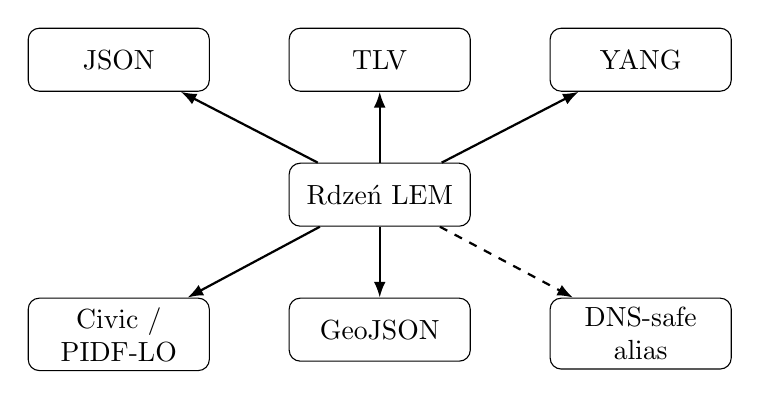
\begin{tikzpicture}[node distance=9mm and 10mm,
  box/.style={draw,rounded corners,align=center,minimum width=23mm,minimum height=8mm},
  arr/.style={-{Latex[length=2mm]},thick}]
  \node[box] (core) {Rdzeń LEM};
  \node[box,above left=of core] (json) {JSON};
  \node[box,above=of core] (tlv) {TLV};
  \node[box,above right=of core] (yang) {YANG};
  \node[box,below left=of core] (civic) {Civic /\\PIDF-LO};
  \node[box,below=of core] (geo) {GeoJSON};
  \node[box,below right=of core] (dns) {DNS-safe\\alias};
  \draw[arr] (core) -- (json);
  \draw[arr] (core) -- (tlv);
  \draw[arr] (core) -- (yang);
  \draw[arr] (core) -- (civic);
  \draw[arr] (core) -- (geo);
  \draw[arr,dashed] (core) -- (dns);
\end{tikzpicture}
\caption{Rdzeń semantyczny i jego reprezentacje oraz mapowania}
\label{fig:lem-representations}
\end{figure}

\section{Reprezentacja tekstowa (Human-readable)}
\label{sec:reprezentacja-tekstowa}
Reprezentacja tekstowa służy do czytelnego przedstawienia informacji o lokalizacji zdefiniowanej przez model LEM.

Reprezentacja tekstowa przedstawia komponenty modelu LEM w formie przeznaczonej do interpretacji przez człowieka. Sposób rozmieszczenia informacji, kolejność występowania komponentów, stosowane separatory lub formatowanie graficzne nie wpływają na znaczenie opisu informacji o lokalizacji.

Znaczenie reprezentacji tekstowej wynika wyłącznie z obecnych komponentów modelu LEM oraz ich interpretacji semantycznej.

\noindent \textbf{Przykład informacyjny:}
\begin{verbatim}
Site: Main Campus
Building: Engineering Center
Level: 2
Reference Space: Room 201
Relative Position: East side
\end{verbatim}

Powyższy zapis przedstawia informację o lokalizacji w sposób czytelny dla człowieka. Konkretna forma prezentacji nie stanowi części modelu semantycznego LEM.

\section{Reprezentacja binarna (Compact / TLV)}
\label{sec:reprezentacja-binarna}
Reprezentacja binarna umożliwia wyrażenie informacji LEM w postaci zwartej struktury danych przeznaczonej do wymiany lub przechowywania informacji.

Mechanizm kodowania binarnego nie definiuje znaczenia informacji o lokalizacji. Znaczenie każdego elementu reprezentacji wynika z odwzorowania na komponenty modelu LEM.

Reprezentacja binarna może wykorzystywać mechanizmy takie jak Type-Length-Value (TLV) --- wzorzec kodowania rozpoznawalny formalnie m.in. z rekomendacji ITU-T X.690 \cite{ITU-X690} (zob. Załącznik B) --- jednak sposób przypisania typów, kodowania wartości oraz organizacji struktury danych należy do określonej specyfikacji reprezentacji lub profilu implementacyjnego.

W reprezentacji binarnej:
\begin{itemize}
    \item typ elementu reprezentacji odpowiada komponentowi modelu LEM,
    \item wartość elementu reprezentacji odpowiada wartości określonego komponentu,
    \item sposób kodowania wartości nie zmienia znaczenia komponentu.
\end{itemize}

Poprawna reprezentacja binarna musi prowadzić do tej samej interpretacji semantycznej, jaka wynikaby z dowolnej innej poprawnej reprezentacji informacji LEM.

\noindent \textbf{Przykład informacyjny} (profil kodowania TLV zdefiniowany poniżej: T = 1 oktet, L = 2 oktety big-endian, V = wartość; \textit{Level} używa jednego oktetu \texttt{kind} oraz czterech oktetów \texttt{int32} dla wartości numerycznej):

\begin{verbatim}
Typ (T)  Nazwa komponentu     Długość (L)  Wartość (V)
0x01     Site                 0x000B       "Main Campus"
0x02     Building             0x0012       "Engineering Center"
0x03     Level                0x0005       0x01 00000002
0x04     Reference Space      0x0007       "Room201"
0x05     Relative Position    0x0009       "East side"
\end{verbatim}

\noindent \textbf{Ciąg oktetów (zapis szesnastkowy):}
\begin{verbatim}
01 00 0B 4D 61 69 6E 20 43 61 6D 70 75 73
02 00 12 45 6E 67 69 6E 65 65 72 69 6E 67 20 43 65 6E 74 65 72
03 00 05 01 00 00 00 02
04 00 07 52 6F 6F 6D 32 30 31
05 00 09 45 61 73 74 20 73 69 64 65
\end{verbatim}

Powyższe przypisanie wartości typu (T) do konkretnego komponentu (np. \texttt{0x03} $\rightarrow$ Level) jest elementem konkretnej specyfikacji reprezentacji lub profilu implementacyjnego, a nie częścią modelu semantycznego LEM --- inny profil binarny może przypisać te same komponenty do innych wartości T, pozostając równoważny semantycznie (zob. 2.4.3), o ile odwzorowanie na komponenty modelu jest jednoznaczne.

\subsection{Formalny rejestr typów (informacyjny)}
\label{sec:rejestr-typow}
Poniższy rejestr formalizuje powyższy przykład:
\begin{enumerate}
    \item Pole L ma 2 oktety, co pozwala opisać pełny zakres długości reprezentacji UTF-8.
    \item Kodowanie Level odzwierciedla strukturę kind+value i wspólną dziedzinę \texttt{int32}.
    \item Relative Position jest zwykłym ciągiem UTF-8, bez podtypu.
\end{enumerate}

\begin{table}[h]
\centering
\small
\begin{tabular}{|l|l|p{8cm}|}
\hline
\textbf{T (1 oktet)} & \textbf{Komponent} & \textbf{Kodowanie wartości (V)} \\ \hline
0x01 & Site & UTF-8 \cite{RFC3629}, 1--1024 oktetów; po dekodowaniu 1--256 punktów kodowych Unicode \\ \hline
0x02 & Building & UTF-8 \cite{RFC3629}, 1--1024 oktetów; po dekodowaniu 1--256 punktów kodowych Unicode \\ \hline
0x03 & Level & 1 oktet kind (0x01=numeric, 0x02=non-building) + dla numeric dokładnie 4 oktety liczby \texttt{int32} ze znakiem, uzupełnienie do dwóch, big-endian; dla non-building brak dalszych oktetów \\ \hline
0x04 & Reference Space & UTF-8 \cite{RFC3629}, 1--1024 oktetów; po dekodowaniu 1--256 punktów kodowych Unicode \\ \hline
0x05 & Relative Position & UTF-8 \cite{RFC3629}, 1--1024 oktetów; po dekodowaniu 1--256 punktów kodowych Unicode \\ \hline
\end{tabular}
\end{table}

\noindent \textbf{Format nagłówka:} T (1 oktet) + L (2 oktety, big-endian, długość V w oktetach) + V.\\
Reguły spójności 2.5.1–2.5.4 stosuje się do zbioru zdekodowanych komponentów dokładnie tak samo, jak w przypadku reprezentacji JSON (zob. 2.5.6).

\section{Reprezentacja JSON}
\label{sec:reprezentacja-json}
Reprezentacja JSON umożliwia wyrażenie informacji LEM przy użyciu struktury danych JSON. JSON stanowi wyłącznie sposób reprezentacji komponentów modelu LEM i nie definiuje własnej semantyki informacji o lokalizacji.

Reprezentacja używa JSON zgodnego z \cite{RFC8259}. Parser MUSI odrzucać obiekty zawierające zduplikowane nazwy właściwości rdzenia, zanim zostanie utworzona postać kanoniczna.

Struktura JSON musi umożliwiać jednoznaczne odwzorowanie elementów reprezentacji na komponenty modelu LEM.

Nazwy właściwości, struktura obiektu oraz sposób kodowania wartości są elementami reprezentacji i nie mogą zmieniać znaczenia komponentów zdefiniowanych w modelu LEM.

Dwa dokumenty JSON są semantycznie równoważne, jeżeli ich interpretacja prowadzi do tej samej interpretacji kanonicznej modelu LEM.

Różnice w:
\begin{itemize}[noitemsep,topsep=2pt]
    \item kolejności właściwości obiektu JSON,
    \item sposobie formatowania dokumentu,
    \item technicznej reprezentacji wartości, jeżeli zachowana jest równoważność znaczenia,
\end{itemize}
nie wpływają na równoważność semantyczną informacji.

\noindent \textbf{Przykład informacyjny:}
\begin{verbatim}
{
  "site": "Main Campus",
  "building": "Engineering Center",
  "level": { "kind": "numeric", "value": 2 },
  "referenceSpace": "Room201",
  "relativePosition": "East side"
}
\end{verbatim}

Poniższy dokument jest semantycznie równoważny powyższemu (inna kolejność właściwości, inne formatowanie):
\begin{verbatim}
{
  "level": { "value": 2, "kind": "numeric" },
  "site": "Main Campus",
  "relativePosition": "East side",
  "referenceSpace": "Room201",
  "building": "Engineering Center"
}
\end{verbatim}

Nazwy właściwości użyte powyżej (\texttt{site}, \texttt{building}, \texttt{level} itd.) są elementem konkretnej reprezentacji --- profil lub schemat implementacyjny MOŻE stosować inne nazwy (zob. 3.1, 4.4.4), o ile odwzorowanie na komponenty modelu LEM pozostaje jednoznaczne.

\noindent \textbf{Przykład informacyjny --- przypadek non-building} (zob. 2.1.6): obiekt znajdujący się na dachu budynku:
\begin{verbatim}
{
  "site": "Main Campus",
  "building": "Engineering Center",
  "level": { "kind": "non-building", "value": null },
  "referenceSpace": "Roof"
}
\end{verbatim}

\section{Alias prezentacyjny DNS-safe}
\label{sec:reprezentacja-dns-safe}
Alias DNS-safe umożliwia prezentację wybranego zakresu informacji LEM w środowiskach posiadających ograniczenia charakterystyczne dla nazw DNS \cite{RFC1035}.

Ograniczenia techniczne wynikające z zasad tworzenia nazw DNS nie definiują znaczenia informacji o lokalizacji.

Znaczenie reprezentacji DNS-safe wynika wyłącznie z odwzorowania użytych elementów na komponenty modelu LEM.

Alias DNS-safe może przedstawiać jedynie podzbiór komponentów modelu LEM. Brak możliwości wyrażenia określonego komponentu w danym środowisku nie zmienia znaczenia modelu, lecz oznacza utratę informacji w aliasie.

Zdefiniowana niżej kanonikalizacja tekstu jest stratna, dlatego DNS-safe \textbf{NIE JEST} równoważną ani odwracalną reprezentacją LEM. Jest wyłącznie aliasem prezentacyjnym. System wymagający odtworzenia postaci kanonicznej MUSI przenosić pełną reprezentację LEM innym kanałem lub stosować oddzielne, bezstratne kodowanie z jednoznacznym schematem dekodowania.

\noindent \textbf{Przykład informacyjny:}
\begin{verbatim}
level2.room201.eng-center.main-campus.loc.example.
\end{verbatim}

\subsection{Formalny schemat etykiet (informacyjny)}
\label{sec:schemat-etykiet}
Formalny schemat wprowadza jawne, krótkie prefiksy w każdej etykiecie, niezależne od jej pozycji w nazwie:

\begin{table}[h]
\centering
\small
\begin{tabular}{|l|l|p{7cm}|}
\hline
\textbf{Prefiks} & \textbf{Komponent} & \textbf{Kodowanie rdzenia etykiety} \\ \hline
s- & Site & Kanonikalizowany ciąg znaków \\ \hline
b- & Building & Kanonikalizowany ciąg znaków \\ \hline
l- & Level & \texttt{l-<N>} dla kind="numeric", wartość nieujemna; \texttt{l-n<N>} dla wartości ujemnej; \texttt{l-nb} dla kind="non-building" \\ \hline
r- & Reference Space & Kanonikalizowany ciąg znaków \\ \hline
\end{tabular}
\end{table}

\noindent Relative Position nigdy nie jest reprezentowany w DNS-safe.\\
Struktura pełnej nazwy (notacja ABNF, zgodnie z \cite{RFC5234}):
\begin{verbatim}
lem-dns-name  = *(component-label ".") suffix "."
component-label = prefix "-" label-core
prefix        = "s" / "b" / "l" / "r"
label-core    = 1*61(ALPHA / DIGIT / "-")
suffix        = 1*(dns-label ".") dns-label
\end{verbatim}

Kanonikalizacja wartości tekstowej (Site, Building, Reference Space) do rdzenia etykiety: zamiana na małe litery, zastąpienie spacji i innych znaków spoza \texttt{[a-z0-9]} znakiem \texttt{-}, zwinięcie kolejnych \texttt{-} do jednego, usunięcie \texttt{-} z brzegów. Ta kanonikalizacja jest stratna.

\noindent \textbf{Uwaga:} Punycode \cite{RFC3492} koduje Unicode w etykietach DNS, ale samo jego użycie nie odtwarza informacji utraconych przez usuwanie separatorów, zakres komponentów ani pominięcie \textit{Relative Position}. Bezstratny wariant wymaga osobnej specyfikacji.

\noindent \textbf{Przykład formalny:}
\begin{verbatim}
s-main-campus.b-engineering-center.l-2.r-room201.loc.example.
\end{verbatim}

\noindent \textbf{Przykład z Level ujemnym:}
\begin{verbatim}
s-main-campus.l-n1.r-parking-p1.loc.example.
\end{verbatim}

\noindent \textbf{Przykład z non-building (dach):}
\begin{verbatim}
s-main-campus.b-engineering-center.l-nb.r-roof.loc.example.
\end{verbatim}

\section{Mapowanie do istniejących modeli informacji}
\label{sec:mapowanie-modeli}
Istniejące modele informacji mogą być wykorzystywane do wyrażania wybranych aspektów informacji LEM poprzez zdefiniowane mapowania semantyczne.

Mapowanie do zewnętrznego modelu informacji nie oznacza zastąpienia modelu LEM ani rozszerzenia jego znaczenia.

Zewnętrzny model pełni rolę źródła reprezentacji określonych komponentów, których znaczenie musi być zgodne z interpretacją LEM.

Komponenty zewnętrznego modelu, które nie posiadają odpowiednika w modelu LEM, pozostają informacją dodatkową i nie stanowią części opisu informacji LEM.

\subsection{Mapowanie do modeli YANG}
\label{sec:mapowanie-yang}
Modele YANG mogą być wykorzystywane jako reprezentacja strukturalna komponentów LEM w środowiskach zarządzania sieciowego i systemowego.

\noindent \textbf{Przykład informacyjny --- poglądowy moduł YANG \cite{RFC7950}:}
\begin{verbatim}
module example-lem-location {
  namespace "urn:example:lem-location";
  prefix "lem";
  description
    "Poglądowe odwzorowanie komponentów modelu semantycznego LEM (Rozdział 2)
     na węzły danych YANG. Wyłącznie informacyjne (zob. 3.6.1).
     Struktura Level odzwierciedla 2.1.6 (kind/value).";

  grouping lem-location {
    description "Grupa węzłów odpowiadająca komponentom modelu LEM (zob. 2.1).";

    leaf site {
      type string { length "1..256"; }
      description "Odwzorowanie komponentu LEM: Site (zob. 2.1.6).";
    }

    leaf building {
      type string { length "1..256"; }
      description "Odwzorowanie komponentu LEM: Building (zob. 2.1.6).";
    }

    container level {
      description
        "Odwzorowanie komponentu LEM: Level (zob. 2.1.6). Struktura
         kind/value zamiast prostej liczby całkowitej.";

      leaf kind {
        type enumeration {
          enum numeric { description "Kondygnacja numerowana."; }
          enum non-building { description "Dach, parking naziemny, przestrzeń zewnętrzna itp."; }
        }
        mandatory true;
      }

      leaf value {
        type int32;
        when "../kind = 'numeric'";
        description "Wymagane i całkowite dla kind=numeric; nieobecne dla kind=non-building.";
      }

      must "(kind = 'numeric' and value) or (kind = 'non-building' and not(value))" {
        error-message "Zgodnie z 2.1.6: value wymagane dla kind=numeric, niedozwolone dla kind=non-building.";
      }
    }

    leaf reference-space {
      type string { length "1..256"; }
      description "Odwzorowanie komponentu LEM: Reference Space (zob. 2.1.6).";
    }

    leaf relative-position {
      type string { length "1..256"; }
      description "Odwzorowanie komponentu LEM: Relative Position (zob. 2.1.6) — opis relacyjny.";
      must "../reference-space" {
        error-message "Relative Position obecny bez Reference Space narusza LEM 2.5.3.";
      }
    }
  }

  container device-location {
    description "Przykładowy węzeł konfiguracyjny wykorzystujący grupę lem-location.";
    uses lem-location;
  }
}
\end{verbatim}

\subsection{Mapowanie do modeli Civic Address}
\label{sec:mapowanie-civic}
Modele Civic Address mogą być wykorzystywane do reprezentacji wybranych komponentów opisujących adresowe aspekty informacji o lokalizacji.

\noindent \textbf{Przykład informacyjny --- dokument PIDF-LO civicAddress \cite{RFC5139}:}
\begin{verbatim}
<civicAddress xml:lang="en-US"
 xmlns="urn:ietf:params:xml:ns:pidf:geopriv10:civicAddr">
  <country>US</country>
  <NAM>Main Campus</NAM>
  <BLD>Engineering Center</BLD>
  <FLR>2</FLR>
  <ROOM>Room201</ROOM>
  <LOC>East side</LOC>
</civicAddress>
\end{verbatim}

\begin{table}[h]
\centering
\small
\begin{tabularx}{\textwidth}{|>{\raggedright\arraybackslash}p{2.2cm}|>{\raggedright\arraybackslash}p{3.3cm}|>{\raggedright\arraybackslash}X|}
\hline
\textbf{CAtype} & \textbf{Komponent LEM} & \textbf{Charakter mapowania} \\ \hline
BLD (27) & Building & Odwzorowanie bezpośrednie. \\ \hline
FLR (28) & Level, kind="numeric" & Odwzorowanie dotyczy wyłącznie przypadku kind="numeric". \\ \hline
(brak wprost) & Level, kind="non-building" & Civic Address nie posiada elementu dedykowanego. \\ \hline
ROOM (23) & Reference Space & Odwzorowanie bezpośrednie. \\ \hline
NAM (22) & Site (interpretacja) & Interpretacyjne. \\ \hline
LOC (1) & Relative Position & Semantycznie bliskie, lecz nie identyczne. \\ \hline
\end{tabularx}
\caption{Mapowanie wybranych typów Civic Address \cite{RFC4776} na komponenty LEM}
\end{table}

\subsection{Mapowanie do modeli geospatial}
\label{sec:mapowanie-geospatial}
Modele geospatial mogą być wykorzystywane do wyrażania przestrzennych aspektów informacji o lokalizacji, w szczególności współrzędnych lub odniesień przestrzennych.

\noindent \textbf{Przykład informacyjny --- obiekt GeoJSON \cite{RFC7946}:}
\begin{verbatim}
{
  "type": "Feature",
  "geometry": {
    "type": "Point",
    "coordinates": [-73.961452, 40.808058]
  },
  "properties": {
    "lem:site": "Main Campus",
    "lem:building": "Engineering Center",
    "lem:level": { "kind": "numeric", "value": 2 },
    "lem:referenceSpace": "Room201",
    "lem:relativePosition": "East side"
  }
}
\end{verbatim}

\noindent Prefiks \texttt{lem:} w nazwach właściwości jest konwencją informacyjną. Kolejność współrzędnych \texttt{[longitude, latitude]} jest wymagana przez \cite{RFC7946} §4.

\section{Przykład ilustracyjny (jedna lokalizacja we wszystkich reprezentacjach)}
\label{sec:przyklad-ilustracyjny}
Poniższy przykład przedstawia tę samą informację o lokalizacji wyrażoną kolejno we wszystkich reprezentacjach. Wszystkie poniższe zapisy MUSZĄ prowadzić do tej samej interpretacji kanonicznej (zob. 2.4.5).

\noindent \textbf{Opisywana lokalizacja:} obiekt znajdujący się w budynku "Engineering Center" na kampusie "Main Campus", na drugiej kondygnacji, w pomieszczeniu "Room201", po wschodniej stronie tego pomieszczenia.

\begin{enumerate}
    \item \textbf{Reprezentacja tekstowa (3.2):}
\begin{verbatim}
Site: Main Campus
Building: Engineering Center
Level: 2 (numeric)
Reference Space: Room201
Relative Position: East side
\end{verbatim}

    \item \textbf{Reprezentacja binarna / TLV (3.3, wg formalnego rejestru 3.3.1 — pole L na 2 oktetach):}
\begin{verbatim}
01 00 0B 4D 61 69 6E 20 43 61 6D 70 75 73
02 00 12 45 6E 67 69 6E 65 65 72 69 6E 67 20 43 65 6E 74 65 72
03 00 05 01 00 00 00 02
04 00 07 52 6F 6F 6D 32 30 31
05 00 09 45 61 73 74 20 73 69 64 65
\end{verbatim}

    \item \textbf{Reprezentacja JSON (3.4):}
\begin{verbatim}
{
  "site": "Main Campus",
  "building": "Engineering Center",
  "level": { "kind": "numeric", "value": 2 },
  "referenceSpace": "Room201",
  "relativePosition": "East side"
}
\end{verbatim}

    \item \textbf{Alias prezentacyjny DNS-safe (3.5.1) --- zapis stratny:}
\begin{verbatim}
s-main-campus.b-engineering-center.l-2.r-room201.loc.example.
\end{verbatim}
\end{enumerate}

\section{Przykłady niepoprawnych opisów lokalizacji}
\label{sec:przyklady-niepoprawne}
\begin{itemize}
    \item \textbf{Przykład 1 --- naruszenie spójności relacji przestrzennych (2.5.3):}
\begin{verbatim}
{
  "site": "Main Campus",
  "building": "Engineering Center",
  "level": { "kind": "numeric", "value": 2 },
  "relativePosition": "East side"
}
\end{verbatim}
Obecny jest komponent \textit{Relative Position}, lecz brakuje \textit{Reference Space}.

    \item \textbf{Przykład 2 --- pusty opis lokalizacji (2.4.4):}
\begin{verbatim}
{}
\end{verbatim}

    \item \textbf{Przykład 3 --- naruszenie struktury Level (2.1.6):}
\begin{verbatim}
{
  "site": "Main Campus",
  "level": { "kind": "non-building", "value": 3 }
}
\end{verbatim}
\end{itemize}

% =====================================================================
% Rozdział 4: Profile i zastosowania modelu LEM
% =====================================================================

\chapter{Profile i zastosowania modelu LEM}
\label{chap:profile}

\section{Rola profili LEM}
Profil LEM definiuje sposób zastosowania modelu LEM w określonym środowisku lub domenie.
Profil MOŻE ograniczać zakres wykorzystywanych komponentów oraz określać dodatkowe wymagania implementacyjne, lecz NIE ROZSZERZA modelu semantycznego LEM i NIE DEFINIUJE nowych komponentów informacji o lokalizacji.
Profil określa sposób wykorzystania istniejących komponentów modelu LEM w określonym kontekście zastosowania. Profil nie zmienia znaczenia komponentów modelu ani zasad ich interpretacji.

\section{Zasady definiowania profili}
Profil LEM MUSI spełniać następujące zasady:

\begin{itemize}
    \item \textbf{Zgodność semantyczna:} Profil NIE MOŻE zmieniać znaczenia komponentów modelu LEM ani definiować alternatywnej interpretacji informacji.
    \item \textbf{Ograniczenie zakresu:} Profil MOŻE ograniczać zakres wykorzystywanych komponentów, lecz NIE MOŻE usuwać ich znaczenia z modelu podstawowego.
    \item \textbf{Jednoznaczność wymagań:} Wymagania określone przez profil MUSZĄ wskazywać, które komponenty są wymagane, opcjonalne lub niewykorzystywane w danym zastosowaniu. Status obecności komponentu nie jest tożsamy z regułami obsługi nieznanych rozszerzeń z sekcji 7.7.
    \item \textbf{Niezależność reprezentacji:} Profil MOŻE określać wymagania dotyczące reprezentacji danych, lecz NIE MOŻE uzależniać znaczenia informacji od konkretnego formatu zapisu.
\end{itemize}

\section{Profile domenowe i przykłady zastosowań}
Poniższe podrozdziały opisują przykładowe domeny, w których model LEM może być stosowany. Każdy opis obejmuje zarówno rolę profilu danej domeny (co profil może ograniczać lub wymagać), jak i sposób integracji z systemami tej domeny — te dwa aspekty są ze sobą ściśle powiązane i celowo omawiane łącznie.

We wszystkich poniższych domenach obowiązuje wspólna zasada: integracja z systemem zewnętrznym NIE MOŻE zależeć od konkretnego protokołu, producenta ani technologii; informacja lokalizacyjna przekazywana pomiędzy systemami MUSI zachowywać znaczenie określone przez model semantyczny LEM; a ograniczenia techniczne systemu zewnętrznego nigdy nie stanowią rozszerzenia modelu LEM (zob. 3.1, 4.5). Jeżeli system zewnętrzny wymaga informacji nieposiadających odpowiednika w LEM, informacje te MUSZĄ być traktowane jako dane dodatkowe lub jako element profilu, zgodnie z zasadami niniejszego rozdziału.

\subsection{Infrastruktura sieciowa}
Profil infrastruktury sieciowej definiuje zastosowanie modelu LEM do opisu fizycznej lokalizacji elementów infrastruktury technicznej, takich jak punkty dostępowe, przełączniki, urządzenia IoT, systemy automatyki budynkowej oraz inne elementy wymagające jednoznacznej identyfikacji przestrzennej.

Integracja z systemami sieciowymi może obejmować urządzenia oraz systemy odpowiedzialne za obsługę infrastruktury technicznej — LEM pełni w tym przypadku rolę wspólnej warstwy semantycznej dla informacji o lokalizacji fizycznej urządzeń, natomiast NIE DEFINIUJE sposobu wykrywania urządzeń, zarządzania konfiguracją sieci ani mechanizmów komunikacji sieciowej.

Profil MOŻE określać wymagania dotyczące minimalnego zakresu informacji lokalizacyjnej wymaganej dla zarządzania infrastrukturą techniczną.

\subsection{Zarządzanie infrastrukturą i CMDB}
Profil zarządzania infrastrukturą i CMDB definiuje zastosowanie modelu LEM w systemach ewidencji, inwentaryzacji oraz dokumentacji technicznej zasobów — obejmując monitorowanie zasobów, zarządzanie konfiguracją, utrzymanie infrastruktury oraz automatyzację procesów operacyjnych.

System ewidencyjny MOŻE przechowywać informacje dodatkowe specyficzne dla własnej domeny, jednak informacje te NIE MOGĄ zmieniać interpretacji komponentów LEM. LEM NIE ZASTĘPUJE systemów zarządzania infrastrukturą — definiuje wyłącznie sposób jednoznacznego opisu znaczenia informacji lokalizacyjnej, umożliwiając interoperacyjność pomiędzy systemami o odmiennych strukturach danych.

\subsection{Lokalizacja awaryjna}
Profil usług lokalizacji awaryjnej definiuje zastosowanie modelu LEM w systemach wymagających przekazania informacji o lokalizacji dla celów bezpieczeństwa lub obsługi zdarzeń wymagających określenia fizycznego położenia.

LEM NIE DEFINIUJE usług ratunkowych, procedur bezpieczeństwa publicznego, mechanizmów obsługi zgłoszeń awaryjnych ani metod wyznaczania lokalizacji, i NIE ZASTĘPUJE istniejących standardów oraz systemów przeznaczonych do obsługi usług alarmowych. Rolą LEM jest reprezentacja oraz interpretacja informacji wynikowej dostarczonej przez system lokalizacyjny, zgodnie z zasadami modelu semantycznego określonymi w Rozdziale 2.

Profil MOŻE określać minimalny zakres informacji wymagany dla jednoznacznego określenia lokalizacji w danym środowisku. Ze względu na wagę tej domeny profil ten powinien szczególnie uwzględniać zasady dotyczące prywatności informacji lokalizacyjnej określone w sekcjach 6.3, 6.6 i 6.7.

\subsubsection{4.3.3.1. Przykładowe rozpisanie profilu (informacyjne)}
Poniżej przedstawiono jeden, w pełni rozpisany przykład profilu „Lokalizacja awaryjna” — od wymagań, przez formalny schemat, po przetestowane przykłady zgodne i niezgodne. Ma to charakter wyłącznie ilustracyjny; rzeczywisty profil dla konkretnego wdrożenia powinien zostać ustalony przez podmiot odpowiedzialny za dane środowisko (zob. 4.1).

Wymagania komponentów (zgodnie z zasadą „Jednoznaczność wymagań”, 4.2):

\begin{table}[htbp]
\centering
\begin{tabular}{|l|l|p{7cm}|}
\hline
\textbf{Komponent} & \textbf{Status w profilu} & \textbf{Uzasadnienie} \\ \hline
Building & Wymagany & Zespół ratunkowy musi wiedzieć, do którego budynku się udać. \\ \hline
Level & Wymagany & Kondygnacja jest krytyczna dla nawigacji w budynkach wielopiętrowych. \\ \hline
Reference Space & Wymagany & Pomieszczenie/przestrzeń referencyjna jest minimalną jednostką lokalizacji użyteczną operacyjnie. \\ \hline
Site & Opcjonalny & Istotny wyłącznie w organizacjach wielokampusowych; jeśli obecny, zwiększa jednoznaczność. \\ \hline
Relative Position & Opcjonalny (zalecany) & Zwiększa precyzję w obrębie Reference Space, lecz nie jest niezbędny do podjęcia interwencji. \\ \hline
\end{tabular}
\caption{Wymagania komponentów dla profilu lokalizacji awaryjnej}
\label{tab:emergency_profile}
\end{table}

Statusy w tabeli określają kompletność danych wymaganą przez profil. Nie określają sposobu obsługi nieznanych rozszerzeń reprezentacji.

Formalny schemat (JSON Schema, informacyjny), rozszerzający szkielet strukturalny modelu podstawowego (2.5.6) przez \texttt{allOf}:

\begin{verbatim}
{
  "$schema": "https://json-schema.org/draft/2020-12/schema",
  "$id": "https://w3id.org/lem/1.0/profile/emergency",
  "title": "LEM — profil: Lokalizacja awaryjna (zob. 4.3.3)",
  "allOf": [
    { "$ref": "https://w3id.org/lem/1.0/schema/core" }
  ],
  "required": [
    "building",
    "level",
    "referenceSpace"
  ]
}
\end{verbatim}

Przykład zgodny z profilem:
\begin{verbatim}
{
  "site": "Main Campus",
  "building": "Engineering Center",
  "level": {
    "kind": "numeric",
    "value": 2
  },
  "referenceSpace": "Room201",
  "relativePosition": "East side, near window"
}
\end{verbatim}

Przykład niezgodny z profilem (lecz zgodny z modelem podstawowym LEM):
\begin{verbatim}
{
  "site": "Main Campus",
  "building": "Engineering Center"
}
\end{verbatim}

\textbf{Uwaga dot. weryfikacji.} Powyższy przykład „niezgodny” został celowo tak dobrany, aby zaprezentować regułę z sekcji 4.4.3: zweryfikowany względem szkieletu modelu podstawowego (2.5.6) dokument ten dał wynik POPRAWNE — to w pełni ważny opis LEM (opis częściowy, zob. 2.4.4). Ten sam dokument zweryfikowany względem schematu profilu dał wynik NIEPOPRAWNE, z dwoma konkretnymi błędami: brakiem pól \texttt{level} i \texttt{referenceSpace}. Jest to bezpośrednie potwierdzenie zasady 4.4.3: „Informacja może być poprawną reprezentacją LEM, lecz jednocześnie nie spełniać wymagań konkretnego profilu zastosowania.”

\subsection{Systemy indoor positioning}
Profil systemów indoor positioning definiuje zastosowanie modelu LEM w środowiskach lokalizacji wewnętrznej, w których położenie określane jest względem przestrzeni referencyjnych oraz relacji przestrzennych.

Profil NIE DEFINIUJE technologii wyznaczania pozycji ani metod pomiarowych. Określa wyłącznie sposób wyrażenia informacji lokalizacyjnej zgodnie z modelem LEM. LEM NIE DEFINIUJE metod pomiaru ani algorytmów lokalizacyjnych wykorzystywanych przez systemy dostarczające dane wejściowe.

\subsection{Dokumentacja techniczna}
LEM MOŻE być wykorzystywany do tworzenia spójnych opisów lokalizacji elementów infrastruktury w dokumentacji technicznej, systemach ewidencyjnych oraz narzędziach wspierających utrzymanie infrastruktury.

Informacja zgodna z LEM MOŻE być przechowywana lub prezentowana w różnych systemach dokumentacyjnych przy zachowaniu tej samej interpretacji semantycznej. LEM NIE DEFINIUJE formatów dokumentacji, narzędzi dokumentacyjnych, metod tworzenia dokumentacji ani procesów zarządzania zmianą dokumentacji technicznej.

\subsection{Automatyzacja i orkiestracja}
LEM MOŻE być wykorzystywany jako warstwa semantyczna dla systemów automatyzacji i orkiestracji wymagających dostępu do informacji o lokalizacji elementów infrastruktury. Informacja lokalizacyjna zgodna z LEM MOŻE być wykorzystywana przez systemy zewnętrzne jako dane wejściowe do realizacji procesów automatycznych.

LEM NIE DEFINIUJE mechanizmów automatyzacji, reguł sterowania, logiki orkiestracji ani sposobów wykorzystania informacji lokalizacyjnej przez systemy wykonawcze.

\subsection{Inne domeny}
Model LEM MOŻE być stosowany w innych domenach wymagających jednoznacznej reprezentacji lub wymiany informacji o lokalizacji (np. systemy automatyki budynkowej, systemy bezpieczeństwa, systemy dokumentacji przestrzennej, systemy analityczne, systemy orkiestracji zasobów), jeżeli sposób wykorzystania modelu zachowuje zgodność z zasadami określonymi w niniejszej specyfikacji.

Nowe zastosowania NIE MOGĄ zmieniać znaczenia komponentów modelu LEM ani definiować alternatywnej interpretacji informacji lokalizacyjnej. Wymagania specyficzne dla określonej domeny POWINNY być definiowane poprzez profile LEM zgodnie z zasadami niniejszego rozdziału.

\section{Ograniczenia i wymagania implementacyjne profili}
Profile mogą określać wymagania implementacyjne wynikające ze specyfiki określonej domeny zastosowania. Wymagania te dotyczą sposobu wykorzystania modelu LEM i NIE STANOWIĄ rozszerzenia jego podstawowej semantyki.

\subsection{Minimalny zakres informacji}
Profil MOŻE określać minimalny zestaw komponentów wymaganych do obsługi informacji o lokalizacji zgodnie z danym zastosowaniem. Minimalny zakres informacji określony przez profil NIE ZMIENIA znaczenia komponentów modelu LEM.

\subsection{Wymagane komponenty}
Profil MOŻE określać komponenty modelu, których obecność jest wymagana w określonym zastosowaniu. Wymaganie obecności komponentu wynika z potrzeb konkretnego profilu i NIE OZNACZA, że komponent ten jest obowiązkowy w podstawowym modelu LEM.

\subsection{Reguły walidacji profilu}
Walidacja profilu jest procesem weryfikacji zgodności opisu lokalizacji z wymaganiami określonymi przez dany profil.

Walidacja profilu jest niezależna od podstawowej interpretacji semantycznej modelu LEM. Informacja może być poprawną reprezentacją LEM, lecz jednocześnie nie spełniać wymagań konkretnego profilu zastosowania.

\subsection{Specyficzne schematy danych}
Profile MOGĄ definiować techniczne schematy danych, takie jak JSON Schema, typy pól, ograniczenia wartości, reguły walidacyjne oraz wymagania implementacyjne.

Schematy te określają sposób wykorzystania modelu LEM w konkretnym środowisku i NIE STANOWIĄ rozszerzenia modelu semantycznego LEM.

Poniższy szkielet JSON Schema ma charakter wyłącznie informacyjny i ilustruje, jak profil może formalnie wyrazić wymagania określone prozą w sekcjach 4.4.1–4.4.2:

\begin{verbatim}
{
  "$schema": "https://json-schema.org/draft/2020-12/schema",
  "$id": "https://w3id.org/lem/1.0/profile/network-infrastructure",
  "title": "Przykładowy profil: infrastruktura sieciowa",
  "allOf": [
    { "$ref": "https://w3id.org/lem/1.0/schema/core" },
    {
      "type": "object",
      "required": ["building", "referenceSpace"],
      "not": { "required": ["relativePosition"] }
    }
  ]
}
\end{verbatim}

Zgodność danych z powyższym schematem stanowi walidację zgodności z profilem (zob. 4.4.3, 5.3) i jest niezależna od walidacji podstawowej zgodności semantycznej z modelem LEM określonej w sekcji 2.5.

\section{Zgodność profili z modelem LEM}
Każdy profil MUSI zachować zgodność z modelem semantycznym LEM określonym w Rozdziale 2.

Profil NIE MOŻE:
\begin{itemize}
    \item zmieniać interpretacji komponentów modelu,
    \item definiować alternatywnej semantyki informacji o lokalizacji,
    \item wprowadzać nowych komponentów semantycznych,
    \item traktować ograniczeń technicznych systemu zewnętrznego jako podstawy do rozszerzenia modelu LEM.
\end{itemize}

Zgodność z LEM jest niezależna od zgodności z wymaganiami konkretnego profilu. System MOŻE być poprawną reprezentacją informacji LEM, nawet jeżeli NIE REALIZUJE wymagań określonego profilu zastosowania.

\section{Rozszerzanie i wersjonowanie profili}
Profile LEM mogą ewoluować w czasie w odpowiedzi na zmieniające się wymagania domenowe. Ewolucja profili NIE MOŻE naruszać stabilności semantycznej podstawowego modelu LEM. Ogólne zasady klasyfikacji zmian modelu (korekcyjna / rozszerzająca / semantyczna) określone w Rozdziale 7 stosuje się odpowiednio do ewolucji profili.

\subsection{Dziedziczenie profili}
Profile MOGĄ tworzyć specjalizacje istniejących profili. Profil potomny MOŻE rozszerzać wymagania profilu nadrzędnego, lecz NIE MOŻE: zmieniać znaczenia komponentów odziedziczonych, usuwać interpretacji określonych przez profil nadrzędny, ani naruszać ograniczeń wynikających z profilu nadrzędnego.

\subsection{Kompatybilność wsteczna}
Ewolucja profilu NIE MOŻE prowadzić do zmiany interpretacji komponentów używanych w starszych wersjach profilu. Zmiany profilu powinny umożliwiać zachowanie zgodności istniejących implementacji wszędzie tam, gdzie nie zmienia się podstawowa semantyka modelu LEM.

\subsection{Ewolucja profili domenowych}
Profile domenowe MOGĄ być aktualizowane w odpowiedzi na zmieniające się potrzeby środowisk zastosowania. Aktualizacja profilu MUSI zachować: zgodność z modelem semantycznym LEM, stabilność interpretacji istniejących komponentów oraz możliwość jednoznacznego określenia różnic pomiędzy wersjami profilu.

Ewolucja profili NIE MOŻE wymagać zmian w podstawowym modelu semantycznym LEM, jeżeli potrzeba zmiany wynika wyłącznie z wymagań konkretnej domeny zastosowania.

% =====================================================================
% Rozdział 5: Zagadnienia implementacyjne
% =====================================================================

\chapter{Zagadnienia implementacyjne}
\label{chap:implementacja}

\section{Przetwarzanie reprezentacji}
Implementacja LEM MUSI umożliwiać odwzorowanie danych zapisanych w reprezentacji LEM na komponenty modelu semantycznego.
Proces przetwarzania NIE MOŻE zmieniać interpretacji komponentów określonej w Rozdziale 2. Dotyczy to również opisów częściowych (zob. 2.4.4) — brak komponentu MUSI być odwzorowany jako brak informacji o mniejszej precyzji, a nie interpretowany jako błąd. Zasady postępowania z elementami nierozpoznanymi przez implementację są określone w sekcji 7.7.

\section{Reprezentacja wewnętrzna implementacji}
Implementacja MOŻE stosować wewnętrzne struktury danych różne od reprezentacji wymiany. Wewnętrzna reprezentacja NIE MOŻE wpływać na semantykę informacji LEM.

\section{Walidacja danych}
Implementacja MOŻE wykonywać walidację w następujących zakresach:

\begin{itemize}
    \item poprawność składniowa — zgodność zapisu ze strukturą wymaganą przez reprezentację,
    \item zgodność z regułami reprezentacji — poprawność odwzorowania elementów reprezentacji na komponenty modelu (obejmuje ocenę kompletności danych wymaganej przez daną reprezentację),
    \item zgodność z profilem zastosowania — spełnienie wymagań określonego profilu (zob. 4.4.3).
\end{itemize}

Walidacja NIE MOŻE definiować nowej interpretacji informacji.

\section{Obsługa błędów}
Implementacja MUSI rozróżniać kategorie błędów odpowiadające zakresom walidacji z sekcji 5.3:

\begin{itemize}
    \item błędy składni reprezentacji,
    \item błędy zgodności z regułami reprezentacji,
    \item błędy zgodności z profilem.
\end{itemize}

Sposób techniczny sygnalizowania tych kategorii błędów (kody błędów, mechanizmy raportowania itp.) pozostaje poza zakresem modelu LEM.

Dane niepoprawne lub niejednoznaczne NIE MOGĄ być interpretowane jako poprawna informacja LEM — jest to bezpośrednia konsekwencja zasady jednoznaczności interpretacji określonej w sekcji 2.5.1.

\section{Wersjonowanie i kompatybilność implementacji}
Zmiany implementacyjne NIE MOGĄ powodować zmiany znaczenia komponentów modelu LEM.

Implementacje POWINNY umożliwiać identyfikację wersji używanych reprezentacji oraz zachowanie możliwości przetwarzania danych zgodnych z wcześniejszymi wersjami modelu (zob. Rozdział 7).
% =====================================================================
% Rozdział 6: Zagadnienia bezpieczeństwa i prywatności
% =====================================================================

\chapter{Zagadnienia bezpieczeństwa i prywatności}
\label{chap:bezpieczenstwo}

\section{Zakres odpowiedzialności modelu}
Model LEM definiuje wyłącznie semantykę informacji o lokalizacji oraz zasady jej interpretacji. LEM NIE DEFINIUJE mechanizmów uwierzytelniania, autoryzacji, kontroli dostępu, szyfrowania, ochrony transmisji, retencji danych ani zasad zarządzania informacjami lokalizacyjnymi.

Implementacje wykorzystujące LEM POWINNY zapewniać mechanizmy ochrony danych odpowiednie do wymagań środowiska, w którym model jest stosowany. Model LEM nie definiuje ani nie weryfikuje spełnienia tego wymagania — pozostaje ono w gestii implementacji i środowiska, podobnie jak inne wymagania pozamodelowe określone w sekcji 2.5.5.

Bezpieczeństwo informacji lokalizacyjnej jest zależne od sposobu jej pozyskania, przechowywania, przetwarzania oraz udostępniania przez systemy wykorzystujące model LEM.

\section{Ochrona integralności informacji}
Informacja lokalizacyjna reprezentowana zgodnie z LEM MUSI zachowywać zgodność z interpretacją kanoniczną modelu.

Implementacja NIE MOŻE modyfikować znaczenia komponentów lokalizacji w sposób prowadzący do zmiany ich interpretacji określonej w Rozdziale 2. Każda modyfikacja informacji lokalizacyjnej, która narusza zasady semantyczne określone w modelu LEM, unieważnia zgodność tych danych z modelem.

Mechanizmy zapewniające integralność danych, w tym kontrola zmian, podpisywanie, sumy kontrolne lub inne metody ochrony informacji, pozostają odpowiedzialnością implementacji.

\section{Separacja lokalizacji od identyfikacji}
Model LEM opisuje informację o fizycznej lokalizacji niezależnie od identyfikacji obiektu, użytkownika lub systemu.

LEM NIE DEFINIUJE:
\begin{itemize}
    \item mechanizmów identyfikacji obiektów,
    \item mechanizmów identyfikacji użytkowników,
    \item sposobów powiązania lokalizacji z konkretną osobą lub podmiotem,
    \item zasad zarządzania tożsamością.
\end{itemize}

Powiązanie informacji lokalizacyjnej z identyfikatorami obiektów lub osób jest wykonywane poza modelem LEM i podlega zasadom obowiązującym w danym systemie. Identyfikatory nadane przez systemy zewnętrzne mogą być wykorzystywane przez implementacje LEM wyłącznie jako sposób odwołania się do elementu opisu lokalizacji (zob. A.9) — takie wykorzystanie nie stanowi mechanizmu identyfikacji w rozumieniu modelu LEM ani nie osłabia zasady separacji określonej w niniejszej sekcji.

Implementacje MUSZĄ uwzględniać, że połączenie informacji lokalizacyjnej z innymi danymi może powodować powstanie dodatkowych wymagań bezpieczeństwa lub prywatności.

\section{Zaufanie do źródła informacji lokalizacyjnej}
Model LEM nie określa metod pozyskiwania informacji lokalizacyjnej ani sposobów oceny wiarygodności źródła danych.

LEM NIE DEFINIUJE:
\begin{itemize}
    \item technologii pomiaru lokalizacji,
    \item algorytmów określania położenia,
    \item metod oceny dokładności lub jakości pomiaru,
    \item mechanizmów potwierdzania pochodzenia danych.
\end{itemize}

Implementacja wykorzystująca LEM MOŻE przechowywać dodatkowe informacje dotyczące pochodzenia lub jakości danych, jednak informacje te nie stanowią części podstawowej semantyki modelu LEM, chyba że zostaną określone przez odpowiedny profil zgodny z zasadami Rozdziału 4.

\section{Profile bezpieczeństwa}
Wymagania bezpieczeństwa specyficzne dla określonych środowisk MOGĄ być definiowane poprzez profile bezpieczeństwa lub profile zastosowań zgodne z zasadami określonymi w Rozdziale 4.

Profil bezpieczeństwa:
\begin{itemize}
    \item NIE MOŻE zmieniać znaczenia komponentów modelu LEM,
    \item NIE MOŻE definiować alternatywnej interpretacji informacji lokalizacyjnej,
    \item MOŻE określać wymagania dotyczące ochrony, dostępu lub sposobu wykorzystania informacji.
\end{itemize}

Profile bezpieczeństwa pozostają ograniczeniami dotyczącymi implementacji lub zastosowania modelu, a nie rozszerzeniem semantyki LEM.

\section{Prywatność informacji lokalizacyjnej}
Model LEM jest neutralny względem klasyfikacji prawnej lub organizacyjnej informacji lokalizacyjnej.

LEM NIE OKREŚLA, czy określona informacja lokalizacyjna stanowi dane osobowe, informację poufną lub inną kategorię danych chronionych.

Ocena charakteru informacji oraz zastosowanie odpowiednich mechanizmów ochrony pozostają odpowiedzialnością systemów wykorzystujących model LEM.

Implementacje MUSZĄ uwzględniać wymagania dotyczące prywatności wynikające z obowiązujących regulacji, polityk organizacyjnych oraz charakteru przetwarzanych danych. W szczególności implementacje POWINNY uwzględniać, że nawet ograniczony podzbiór komponentów LEM (np. Reference Space i Relative Position bez pełnego kontekstu hierarchicznego) może, w zależności od kontekstu, stanowić informację o istotnym znaczeniu dla prywatności (zob. 2.4.4).

\section{Minimalizacja ujawnianej informacji}
Systemy wykorzystujące LEM POWINNY ograniczać zakres udostępnianych informacji lokalizacyjnych do poziomu wymaganego przez określony cel zastosowania.

Udostępniana reprezentacja informacji lokalizacyjnej MOŻE wykorzystywać ograniczony zakres komponentów modelu, jeżeli zachowana zostaje zgodność z wymaganiami danego profilu oraz interpretacją semantyczną LEM.

Model LEM nie definiuje polityk ujawniania informacji ani mechanizmów kontroli dostępu. Zasady te pozostają odpowiedzialnością implementacji.

\section{Spójność semantyczna rozszerzeń a bezpieczeństwo}
Rozszerzenia wykorzystujące model LEM MUSZĄ zachowywać zgodność z podstawową semantyką modelu (zob. 3.1, 4.5, 7.4).

Rozszerzenie NIE MOŻE wprowadzać nowych znaczeń istniejących komponentów ani powodować niejednoznaczności interpretacji informacji lokalizacyjnej.

Z punktu widzenia bezpieczeństwa, rozszerzenie niespełniające tej zasady stanowi dodatkowe ryzyko: pole rozszerzenia błędnie zinterpretowane jako standardowy komponent LEM może prowadzić implementację do niepoprawnego wniosku o lokalizacji obiektu. Implementacje POWINNY jednoznacznie odróżniać dane rozszerzeń od komponentów podstawowych modelu LEM podczas przetwarzania (zob. 5.1, 7.7).

Dodatkowe informacje wymagane przez określone środowisko zastosowania POWINNY być definiowane poprzez mechanizmy rozszerzeń lub profile, a nie poprzez zmianę podstawowego modelu semantycznego LEM.

\section{Zbiorczy model zagrożeń (informacyjny)}
Poniższa tabela zestawia w jednym miejscu zagrożenia, których dotyczą zasady rozproszone w sekcjach 6.1–6.8, wraz z mechanizmami obrony — pozostającymi, zgodnie z 6.1, poza zakresem modelu LEM. Ma charakter informacyjny i poglądowy, a nie wyczerpującej, formalnej analizy zagrożeń.

\begin{table}[p]
\centering
\footnotesize
\setlength{\tabcolsep}{3pt}
\begin{tabular}{|p{0.35cm}|p{1.9cm}|p{2.3cm}|p{2.5cm}|p{2.5cm}|p{0.75cm}|}
\hline
\textbf{Nr} & \textbf{Zagrożenie} & \textbf{Wektor} & \textbf{Konsekwencja} & \textbf{Mechanizm obrony (poza zakresem LEM)} & \textbf{Odn.} \\ \hline
1 & Podsłuch transmisji & Przechwycenie danych lokalizacyjnych podczas przesyłania między systemami & Ujawnienie lokalizacji osobom nieuprawnionym & Szyfrowanie transportu (np. TLS) & 6.1 \\ \hline
2 & Naruszenie integralności w tranzycie & Modyfikacja wartości komponentów bez wykrycia & Błędna interpretacja lokalizacji — szczególnie krytyczne w profilu lokalizacji awaryjnej (4.3.3) & Podpisywanie, sumy kontrolne & 6.2 \\ \hline
3 & Fałszowanie źródła danych & Wstrzyknięcie danych z podszywającego się lub niezaufanego źródła & Zaufanie do nieprawdziwej lokalizacji & Uwierzytelnianie źródła & 6.4 \\ \hline
4 & Deanonimizacja przez korelację & Połączenie informacji lokalizacyjnej z identyfikatorem zewnętrznym lub wzorcem & Ujawnienie tożsamości osoby mimo formalnej separacji lokalizacja $\leftrightarrow$ identyfikacja & Kontrola dostępu, ograniczenie łączenia zbiorów danych & 6.3, 6.6 \\ \hline
5 & Nadmierne ujawnienie precyzji & Udostępnienie pełnego, precyzyjnego opisu lokalizacji tam, gdzie cel wymagał mniejszej precyzji & Ujawnienie więcej informacji niż niezbędne do celu & Minimalizacja zakresu ujawnianych komponentów & 6.7, 2.4.4 \\ \hline
6 & Wstrzyknięcie nierozpoznanego rozszerzenia & Dodanie pola o nazwie/strukturze imitującej komponent LEM & Błędna interpretacja danych rozszerzenia jako części modelu semantycznego & Jawne, techniczne rozróżnianie rozszerzeń od komponentów podstawowych & 6.8, 5.1 \\ \hline
7 & Obejście wymagań profilu & Świadome przesłanie opisu zgodnego z modelem podstawowym, lecz nie spełniającego wymagań profilu & Działanie na podstawie informacji o niewystarczającej precyzji & Wymuszenie walidacji zgodności z profilem po stronie odbiorcy & 4.4.3, 4.3.3.1 \\ \hline
8 & Wykorzystanie nieaktualnych danych & Odebranie i wykorzystanie przestarzałego stanu informacji lokalizacyjnej & Działanie na podstawie nieaktualnej lokalizacji obiektu & Znaczniki czasu, mechanizmy świeżości danych & A.12, 6.4 \\ \hline
\end{tabular}
\caption{Zbiorczy model zagrożeń (informacyjny)}
\label{tab:threat_model}
\end{table}

Pozycje 6 i 7 wynikają bezpośrednio z właściwości modelu LEM opisanych w innych rozdziałach (odpowiednio: rozróżnianie rozszerzeń od komponentów podstawowych oraz niezależność walidacji profilu od walidacji modelu podstawowego) i ilustrują, że dyscyplina semantyczna modelu ma również praktyczne konsekwencje dla bezpieczeństwa, a nie wyłącznie dla spójności interpretacji.

% =====================================================================
% Rozdział 7: Ewolucja, rozszerzanie i wersjonowanie modelu LEM
% =====================================================================

\chapter{Ewolucja, rozszerzanie i wersjonowanie modelu LEM}
\label{chap:ewolucja}

\section{Klasyfikacja zmian modelu}
Zmiany dotyczące modelu LEM MUSZĄ być klasyfikowane według ich wpływu na semantykę modelu. Poniższa klasyfikacja dotyczy zmian w modelu podstawowym; zasady ewolucji samych profili określa sekcja 4.6, która odwołuje się odpowiednio do niniejszej klasyfikacji.

Wyróżnia się następujące typy zmian:

\subsection{Zmiana korekcyjna}
Zmiana korekcyjna usuwa niejednoznaczności, błędy dokumentacyjne lub poprawia opis istniejących elementów modelu.

Zmiana korekcyjna NIE MOŻE zmieniać interpretacji komponentów modelu LEM ani wpływać na zgodne implementacje istniejących wersji.

\subsection{Zmiana rozszerzająca}
Zmiana rozszerzająca wprowadza nowe możliwości modelu przy zachowaniu istniejącej semantyki.

Zmiana rozszerzająca MOŻE obejmować: dodanie nowych komponentów, dodanie nowych opcjonalnych właściwości, rozszerzenie zakresu obsługiwanych reprezentacji, dodanie nowych profili zastosowań.

Zmiana rozszerzająca NIE MOŻE powodować zmiany znaczenia istniejących komponentów modelu LEM.

\subsection{Zmiana semantyczna}
Zmiana semantyczna wpływa na podstawowe znaczenie elementów modelu LEM.

Przykłady zmian semantycznych obejmują: zmianę definicji istniejącego komponentu, zmianę relacji pomiędzy komponentami, zmianę zasad interpretacji kanonicznej, zmianę zasad określania równoważności semantycznej.

Zmiana semantyczna MUSI być traktowana jako zmiana podstawowej wersji modelu LEM.

\section{Zasady wersjonowania}
Wersjonowanie LEM MUSI umożliwiać jednoznaczne określenie zgodności pomiędzy implementacjami wykorzystującymi model.

Wersjonowanie powinno rozróżniać: wersję modelu semantycznego LEM, wersję zasad reprezentacji oraz wersję profili zastosowań.

Zmiana wersji reprezentacji lub profilu NIE MOŻE powodować zmiany podstawowej semantyki modelu LEM.

\section{Kompatybilność wersji}
Implementacje LEM MUSZĄ określać wersję modelu semantycznego, według której interpretowane są dane lokalizacyjne.

Dwie implementacje są zgodne semantycznie, jeżeli:
\begin{itemize}
    \item wykorzystują zgodną wersję modelu semantycznego LEM,
    \item interpretują komponenty zgodnie z tym samym modelem znaczeniowym,
    \item zachowują zasady interpretacji kanonicznej.
\end{itemize}

Różnice w wersjach reprezentacji lub profili mogą być obsługiwane niezależnie od wersji rdzenia semantycznego, o ile zachowana jest zgodność interpretacji.

\section{Zasady rozszerzania modelu}
Rozszerzenia modelu LEM MUSZĄ zachowywać istniejącą semantykę komponentów podstawowych.

Nowy komponent lub właściwość:
\begin{itemize}
    \item NIE MOŻE zmieniać znaczenia istniejących komponentów,
    \item NIE MOŻE powodować alternatywnej interpretacji istniejących danych,
    \item MUSI posiadać jednoznacznie określone znaczenie.
\end{itemize}

Jeżeli wymagane jest wprowadzenie nowego znaczenia informacji lokalizacyjnej, zmiana MUSI zostać wykonana w modelu podstawowym LEM, a nie poprzez profil lub implementację lokalną.

Niniejsza sekcja dotyczy rozszerzeń przeznaczonych do formalnego włączenia do modelu LEM. Rozszerzenia o charakterze lokalnym, niepodlegające takiemu włączeniu, opisuje sekcja 7.5.

\section{Rozszerzenia prywatne i domenowe}
Implementacje MOGĄ definiować rozszerzenia lokalne lub domenowe, przeznaczone wyłącznie do użytku w określonym środowisku i niepodlegające formalnemu włączeniu do modelu podstawowego, jeżeli rozszerzenia te:
\begin{itemize}
    \item nie zmieniają znaczenia komponentów zdefiniowanych przez LEM,
    \item nie powodują niejednoznacznej interpretacji danych zgodnych z LEM,
    \item są wyraźnie oddzielone od podstawowego modelu LEM.
\end{itemize}

Rozszerzenia lokalne NIE MOGĄ być traktowane jako standardowe komponenty LEM bez formalnego włączenia ich do modelu zgodnie z zasadami sekcji 7.4.

\section{Proces zmian semantycznych}
Zmiany wpływające na podstawową semantykę modelu LEM MUSZĄ podlegać szczególnej procedurze wersjonowania.

Procedura ta MUSI zapewniać: identyfikację zakresu zmiany, określenie wpływu na istniejące implementacje, określenie zasad migracji oraz zachowanie możliwości interpretacji starszych danych.

Zmiana semantyczna NIE MOŻE być wprowadzona wyłącznie poprzez zmianę reprezentacji lub profilu zastosowania.

Sposób prowadzenia tego procesu w praktyce (np. organ decyzyjny, tryb konsultacji, publikacja zmian) pozostaje poza zakresem modelu LEM.

\section{Obsługa nieznanych elementów}
Implementacje LEM MUSZĄ rozróżniać elementy nieznane według ich znaczenia dla interpretacji danych. To, czy dany element ma dla implementacji charakter opcjonalny czy krytyczny, jest ustalane kontekstowo — na podstawie wymagań profilu zastosowania (zob. 4.2, 4.4.2), a nie odgórnie przez sam model LEM.

\subsection{Element opcjonalny}
Element opcjonalny, którego brak nie wpływa na interpretację podstawowej informacji lokalizacyjnej, MOŻE zostać pominięty przez implementację.

\subsection{Element krytyczny}
Element krytyczny, którego znaczenie jest wymagane do poprawnej interpretacji informacji lokalizacyjnej, NIE MOŻE zostać pominięty.

Implementacja, która nie obsługuje elementu krytycznego, MUSI oznaczyć dane jako nieinterpretowalne lub niezgodne z obsługiwaną wersją modelu (zob. 5.4).

\section{Stabilność modelu LEM}
Rozwój modelu LEM MUSI zachowywać stabilność podstawowej semantyki.

Zmiany modelu powinny preferować: rozszerzanie zamiast redefinicji, dodawanie nowych możliwości zamiast zmiany istniejących znaczeń, zachowanie kompatybilności istniejących danych.

Podstawowym celem procesu ewolucji LEM jest zachowanie możliwości jednoznacznej interpretacji informacji lokalizacyjnej w kolejnych wersjach modelu.
% =====================================================================
% Rozdział 8: Prace powiązane i pozycjonowanie modelu
% =====================================================================

\chapter{Prace powiązane i pozycjonowanie modelu}
\label{chap:related-work}

LEM dotyczy obszaru, w którym funkcjonują dojrzałe standardy lokalizacyjne i modele budynkowe. Celem niniejszego rozdziału nie jest zastąpienie tych rozwiązań, lecz wyznaczenie granicy zakresu proponowanego modelu.

\section{Standardy informacji lokalizacyjnej}
PIDF-LO definiuje obiekt lokalizacji przenoszony w dokumencie obecności i obejmuje informacje geodezyjne oraz civic \cite{RFC4119,RFC5139}. RFC~5491 dodatkowo ogranicza użycie PIDF-LO w celu poprawy interoperacyjnej interpretacji \cite{RFC5491}. LEM ma węższy cel: nie definiuje dokumentu obecności, polityki użycia ani geometrii, lecz pięcioskładnikowy rdzeń lokalizacji i mapowania reprezentacyjne.

IndoorGML~2.0 jest rozbudowanym modelem konceptualnym przestrzeni wewnętrznych, topologii, łączności i nawigacji \cite{IndoorGML2025}. IndoorLocationGML proponuje natomiast ramy kodowania lokalizacji absolutnej i względnej w środowisku indoor \cite{IndoorLocationGML2016}. W porównaniu z tymi rozwiązaniami LEM nie aspiruje do modelowania geometrii ani tras; może służyć jako mały opis lokalizacyjny na granicy systemów, które przechowują bogatszy model przestrzeni.

\section{Semantyczne modele budynków}
Brick jest ontologią metadanych dla przenośnych aplikacji inteligentnych budynków i modeluje m.in. zasoby, przestrzenie oraz relacje lokalizacyjne \cite{Brick2018}. Project Haystack definiuje konwencje tagowania obejmujące hierarchię site, space, floor i room oraz numery kondygnacji \cite{HaystackSpaces2026}. Oba rozwiązania oferują bogatszy opis zasobów i relacji budynkowych. LEM koncentruje się na przenośnym opisie samej lokalizacji encji, niezależnym od pełnej ontologii systemu źródłowego.

\section{Porównanie zakresu}
Tabela \ref{tab:related-comparison} porównuje zakresy, a nie dojrzałość ani jakość rozwiązań. Określenie „częściowo” oznacza, że cecha występuje w innej strukturze lub jako część szerszego modelu.

\begin{table}[htbp]
\centering
\footnotesize
\setlength{\tabcolsep}{3pt}
\begin{tabularx}{\textwidth}{|>{\raggedright\arraybackslash}X|c|c|c|c|c|}
\hline
\textbf{Cecha} & \textbf{LEM} & \textbf{PIDF-LO} & \textbf{IndoorGML} & \textbf{Brick} & \textbf{Haystack} \\ \hline
Mały rdzeń niezależny od formatu & tak & nie & nie & nie & nie \\ \hline
Geometria / współrzędne & mapowanie & tak & tak & częściowo & częściowo \\ \hline
Topologia i nawigacja indoor & nie & nie & tak & częściowo & częściowo \\ \hline
Hierarchia site/building/level/space & tak & częściowo & tak & tak & tak \\ \hline
Opis położenia względnego tekstem & tak & częściowo & tak & częściowo & częściowo \\ \hline
Opisy częściowe i profile wymagań & tak & reguły użycia & rozszerzenia & rozszerzenia & konwencje \\ \hline
Łączne mapowania JSON/YANG/TLV & tak & nie & nie & nie & nie \\ \hline
Ścisła równość postaci kanonicznej & tak & inny model & inny model & tożsamość grafu & konwencje \\ \hline
\end{tabularx}
\caption{Porównanie zakresu LEM i wybranych rozwiązań powiązanych}
\label{tab:related-comparison}
\end{table}

\section{Granica deklarowanej nowości}
Deklarowany wkład LEM polega na połączeniu: małego pięcioskładnikowego rdzenia, dokładnej krotki kanonicznej, opisów częściowych, profili oraz zestawu mapowań dla środowisk sieciowych i zarządczych. Dokument nie twierdzi, że wprowadza pierwszą reprezentację lokalizacji wewnętrznej ani że zastępuje PIDF-LO, IndoorGML, Brick lub Haystack.

Niniejsza wersja jest specyfikacją techniczną. Artefakty referencyjne potwierdzają spójność składniową schematów i przykładów, lecz nie stanowią jeszcze eksperymentalnej oceny interoperacyjności pomiędzy niezależnymi implementacjami. Taka ocena pozostaje zadaniem dla dalszej pracy badawczej.


% =====================================================================
% ZAŁĄTNIKI
% =====================================================================
\appendix
% =====================================================================
% Załącznik A: Glosariusz terminów LEM
% =====================================================================

\appendix
\chapter{Glosariusz terminów LEM}
\label{app:glosariusz}

\section{Terminy normatywne}
Terminy zdefiniowane w niniejszym glosariuszu mają znaczenie normatywne dla całej specyfikacji LEM. Użycie terminu zdefiniowanego w glosariuszu MUSI być zgodne z jego znaczeniem określonym w niniejszym załączniku.

Model LEM opisuje znaczenie informacji lokalizacyjnej, a nie: sposób identyfikacji obiektów, sposób pozyskiwania informacji lokalizacyjnej, metodę określania położenia, sposób przechowywania historii zmian, mechanizmy bezpieczeństwa lub zarządzania dostępem.

Rozszerzenia, profile oraz implementacje LEM NIE MOGĄ wprowadzać nowych znaczeń dla istniejących terminów ani komponentów modelu. W przypadku konieczności wprowadzenia nowego znaczenia semantycznego zmiana MUSI zostać wykonana w podstawowym modelu LEM zgodnie z zasadami wersjonowania określonymi w Rozdziale 7.

\section{Zestawienie pojęć}
Poniższa tabela zawiera definicje kluczowych terminów modelu LEM.

\footnotesize
\setlength{\tabcolsep}{4pt}
\renewcommand{\arraystretch}{1.3}
\begin{longtable}{|p{0.27\textwidth}|p{0.68\textwidth}|}
\caption{Glosariusz terminów modelu LEM}\label{tab:glossary}\\
\hline
\textbf{Termin} & \textbf{Definicja} \\ \hline
\endfirsthead
\hline
\textbf{Termin} & \textbf{Definicja} \\ \hline
\endhead
\textbf{A.1. Lokalizacja} \newline (Location) & Informacja opisująca położenie obiektu względem jednej lub wielu przestrzeni referencyjnych. Lokalizacja stanowi semantyczny opis relacji przestrzennych, hierarchicznych lub innych określonych przez model LEM. LEM nie definiuje metod pomiaru ani sposobów pozyskiwania informacji lokalizacyjnej. \\ \hline
\textbf{A.2. Obiekt} \newline (Object / Entity) & Element fizyczny lub logiczny opisywany przez model LEM. Tożsamość obiektu jest zarządzana przez systemy zewnętrzne. LEM nie definiuje mechanizmów tworzenia, nadawania ani zarządzania identyfikatorami obiektów. \\ \hline
\textbf{A.3. Komponent} \newline (Component) & Element modelu LEM posiadający określone i jednoznaczne znaczenie semantyczne. Zbiór komponentów modelu LEM jest zamknięty i definiowany przez specyfikację modelu (zob. 2.1). Rozszerzenia nie mogą zmieniać znaczenia istniejących komponentów. \\ \hline
\textbf{A.4. Przestrzeń referencyjna} \newline (Reference Space) & Obiekt lub przestrzeń posiadająca rolę referencyjną (zob. A.11) i stanowiąca element odniesienia dla opisu lokalizacji. Przestrzeń referencyjna może reprezentować dowolny element przestrzeni fizycznej lub logicznej, jeżeli spełnia wymagania interpretacji modelu LEM. Komponenty Site, Building i Level są nazwanymi realizacjami tej roli w kontekście hierarchicznym (zob. 2.1). \\ \hline
\textbf{A.5. Położenie względne} \newline (Relative Position) & Informacja określająca położenie obiektu względem określonej przestrzeni referencyjnej lub elementu posiadającego rolę referencyjną. Położenie względne jest interpretowane zgodnie z zasadami modelu LEM i nie definiuje sposobu określania położenia. \\ \hline
\textbf{A.6. Relacja} \newline (Relation) & Kierunkowy związek semantyczny pomiędzy elementami modelu LEM. Relacja określa sposób interpretacji zależności pomiędzy elementami. Kierunek relacji jest częścią jej znaczenia i nie może być pomijany podczas interpretacji informacji (zob. A.13). \\ \hline
\textbf{A.7. Reprezentacja} \newline (Representation) & Forma zapisu informacji zgodnej z modelem LEM, przeznaczona do przechowywania, wymiany lub przetwarzania danych. Reprezentacja może być tekstowa, binarna lub strukturalna. Różne reprezentacje są równoważne semantycznie, jeżeli prowadzą do tej samej interpretacji informacji określonej przez model LEM w zakresie reprezentowanych komponentów. \\ \hline
\textbf{A.8. Interpretacja kanoniczna} \newline (Canonical Interpretation) & Jednoznaczne znaczenie informacji wynikające z zasad modelu LEM, niezależne od zastosowanej reprezentacji danych. Interpretacja kanoniczna określa sposób rozumienia informacji, a nie jej fizyczny sposób zapisu. \\ \hline
\textbf{A.9. Identyfikacja} \newline (Identification) & Proces przypisania oznaczenia lub identyfikatora obiektowi albo przestrzeni przez system zewnętrzny. LEM nie definiuje mechanizmów identyfikacji obiektów ani przestrzeni referencyjnych. Identyfikatory nadane poza modelem LEM mogą być wykorzystywane przez implementacje LEM wyłącznie jako sposób odwołania się do elementów opisu lokalizacji — takie wykorzystanie nie stanowi mechanizmu identyfikacji w rozumieniu LEM (zob. 6.3). \\ \hline
\textbf{A.10. Profil} \newline (Profile) & Ograniczenie lub specjalizacja modelu LEM przeznaczona dla określonej domeny zastosowania. Profil może definiować wymagania dotyczące wykorzystania komponentów i reprezentacji, lecz nie może zmieniać podstawowej semantyki modelu LEM. \\ \hline
\textbf{A.11. Rola referencyjna} \newline (Reference Role) & Zdolność obiektu lub elementu modelu do pełnienia funkcji przestrzeni odniesienia w określonym kontekście interpretacji. Rola referencyjna nie zmienia podstawowej klasyfikacji elementu, lecz określa sposób jego wykorzystania w modelu lokalizacji. Site, Building, Level i Reference Space są komponentami pełniącymi tę rolę (zob. 2.1). \\ \hline
\textbf{A.12. Stan informacji lokalizacyjnej} \newline (Location Information State) & Reprezentacja relacji lokalizacyjnych obowiązujących w momencie interpretacji informacji. Model LEM opisuje stan informacji lokalizacyjnej i nie definiuje mechanizmów zarządzania historią zmian, znaczników czasu ani rejestracji zdarzeń. \\ \hline
\textbf{A.13. Relacja kierunkowa} \newline (Directed Relation) & Relacja, w której kolejność elementów uczestniczących w relacji stanowi część znaczenia semantycznego. Relacja \texttt{located\_in(Object, ReferenceSpace)} posiada inne znaczenie niż relacja odwrotna \texttt{contains(ReferenceSpace, Object)} (zob. 2.2). \\ \hline
\end{longtable}


% --- Bibliografia ---------------------------------------------------
\bibliographystyle{plain}
{\raggedright\sloppy\small\bibliography{bibliography}}

\end{document}
